%%%%%%%%%%%%%%%%
% Ph.D. thesis %
%%%%%%%%%%%%%%%%

%\documentclass[11pt,openright,twoside,letterpaper,onecolumn]{report} %% USE THIS FOR DOUBLE SIDED
\documentclass[11pt,openright,oneside,letterpaper,onecolumn]{report}  %% USE THIS FOR SINGLE SIDED

\usepackage{graphics}
%\usepackage{epsfig}
%%\usepackage{times}
%\usepackage{amsmath}
\usepackage{xspace}
\usepackage[nolineno,noindent,norules]{lgrind}
\usepackage{subfig,graphics,graphicx,color}
\usepackage{pifont}
%\DeclareGraphicsExtensions{.eps}

%%%
%%% Packages
%%%
\usepackage[dvips]{epsfig}
\usepackage{amsmath}
\usepackage{named}
\usepackage{fancyhdr}
\usepackage{afterpage}

%%\makeatletter
%%\def\v#1{{\mbox{\fontfamily{cmtt}\fontsize{\f@size}{\f@size}\selectfont #1}}}
%%\let\v\texttt
\let\vv\texttt

%% Title stuff.
\newcommand{\mykeywords}[0]{Deterministic Multithreading, Stable 
Multithreading, Reliability, Security, Software Model Checking,
State Space Reduction, State Machine Replication}

\newcommand{\thesistitle}{Stable Multithreading: A New Paradigm for Reliable and Secure Threads}
\newcommand{\thesisauthor}{Heming Cui}
\newcommand{\thesisyear}{2015}

%% Systems and techniques names.
\newcommand{\dmt}[0]{\mbox{DMT}\xspace}
\newcommand{\smt}[0]{\mbox{StableMT}\xspace}
\newcommand{\tern}[0]{\mbox{\textsc{Tern}}\xspace}
\newcommand{\peregrine}[0]{\mbox{\textsc{Peregrine}}\xspace}
\newcommand{\parrot}[0]{\mbox{\textsc{Parrot}}\xspace}
\newcommand{\crane}[0]{\mbox{\textsc{Crane}}\xspace}

\newcommand{\racepro}[0]{\textsc{RacePro}\xspace}
\newcommand{\grace}[0]{Grace\xspace}
\newcommand{\coredet}[0]{\textsc{CoreDet}\xspace}
\newcommand{\kendo}[0]{Kendo\xspace}
\newcommand{\dthreads}[0]{\textsc{DThreads}\xspace}
\newcommand{\determinator}[0]{Determinator\xspace}
\newcommand{\dbug}[0]{\textsc{dbug}\xspace}
\newcommand{\ecosys}[0]{\parrot-\dbug}
\newcommand{\paxos}[0]{\textsc{Paxos}\xspace}
\newcommand{\threadsanitizer}[0]{ThreadSanitizer\xspace}
\newcommand{\X}[0]{$\times$\xspace}

%% Application names.
\newcommand{\http}{HTTP\xspace}
\newcommand{\apache}{\vv{Apache}\xspace}
\newcommand{\ab}{\vv{ApacheBench}\xspace}
\newcommand{\mysql}{\vv{MySQL}\xspace}
\newcommand{\sysbench}{\vv{SysBench}\xspace}
\newcommand{\mplayer}[0]{{MPlayer}\xspace}
\newcommand{\mencoder}[0]{\vv{mencoder}\xspace}
\newcommand{\pbzip}[0]{\vv{PBZip2}\xspace}
\newcommand{\aget}[0]{\vv{aget}\xspace}
\newcommand{\mongoose}[0]{\vv{Mongoose}\xspace}
\newcommand{\pfscan}[0]{\vv{pfscan}\xspace}
\newcommand{\fft}[0]{\vv{fft}\xspace}
\newcommand{\lu}[0]{\vv{lu}\xspace}
\newcommand{\luc}[0]{\vv{lu\_cb}\xspace}
\newcommand{\lun}[0]{\vv{lu\_ncb}\xspace}
\newcommand{\barnes}[0]{\vv{barnes}\xspace}
\newcommand{\radix}[0]{\vv{radix}\xspace}
\newcommand{\radiosity}[0]{\vv{radiosity}\xspace}
\newcommand{\waters}[0]{\vv{water-spatial}\xspace}
\newcommand{\watern}[0]{\vv{water-nsquared}\xspace}
\newcommand{\oceanncp}[0]{\vv{ocean}\xspace}
\newcommand{\oceancp}[0]{\vv{ocean}\xspace}
\newcommand{\ocean}[0]{\vv{ocean}\xspace}
\newcommand{\fmm}[0]{\vv{fmm}\xspace}
\newcommand{\volrend}[0]{\vv{volrend}\xspace}
\newcommand{\cholesky}[0]{\vv{cholesky}\xspace}
\newcommand{\streamcluster}[0]{\vv{streamcluster}\xspace}
\newcommand{\blackscholes}[0]{\vv{blackscholes}\xspace}
\newcommand{\swaptions}[0]{\vv{swaptions}\xspace}
\newcommand{\bodytrack}[0]{\vv{bodytrack}\xspace}
\newcommand{\bodytrackopenmp}[0]{\vv{bodytrack-openmp}\xspace}
\newcommand{\ferret}[0]{\vv{ferret}\xspace}
\newcommand{\dedup}[0]{\vv{dedup}\xspace}
\newcommand{\raytrace}[0]{\vv{raytrace}\xspace}
\newcommand{\canneal}[0]{\vv{canneal}\xspace}
\newcommand{\racey}[0]{\vv{racey}\xspace}
\newcommand{\freqmine}[0]{\vv{freqmine}\xspace}
\newcommand{\vips}[0]{\vv{vips}\xspace}
\newcommand{\xtwosixfour}[0]{\vv{x264}\xspace}
\newcommand{\fluidanimate}[0]{\vv{fluidanimate}\xspace}
\newcommand{\facesim}[0]{\vv{facesim}\xspace}
\newcommand{\rtviewraytrace}[0]{\vv{rtview\_raytrace}\xspace}
\newcommand{\wordcount}[0]{\vv{word\_count}\xspace}
\newcommand{\klee}[0]{\textsc{klee}\xspace}
\newcommand{\woodpecker}[0]{\textsc{woodpecker}\xspace}
\newcommand{\splashx}[0]{\mbox{SPLASH-2x}\xspace}
\newcommand{\splash}[0]{\mbox{SPLASH-2}\xspace}
\newcommand{\parsec}[0]{\mbox{PARSEC}\xspace}
\newcommand{\phoenix}[0]{\mbox{Phoenix}\xspace}
\newcommand{\pthread}[0]{\mbox{Pthreads}\xspace}

%% Application names (continue).
\newcommand{\kmeans}[0]{\vv{kmeans}\xspace}
\newcommand{\kmeanspthread}[0]{\vv{kmeans-pthread}\xspace}
\newcommand{\linearregre}[0]{\vv{linear-regression}\xspace}
\newcommand{\linearregrepthread}[0]{\vv{linear-regression-pthread}\xspace}
\newcommand{\matrixmult}[0]{\vv{matrix-multiply}\xspace}
\newcommand{\matrixmultpthread}[0]{\vv{matrix-multiply-pthread}\xspace}
\newcommand{\wordcnt}[0]{\vv{word-count}\xspace}
\newcommand{\wordcntpthread}[0]{\vv{word-count-pthread}\xspace}
\newcommand{\stringmatch}[0]{\vv{string-match}\xspace}
\newcommand{\stringmatchpthread}[0]{\vv{string-match-pthread}\xspace}
\newcommand{\histogram}[0]{\vv{histogram}\xspace}
\newcommand{\histogrampthread}[0]{\vv{histogram-pthread}\xspace}
\newcommand{\pca}[0]{\vv{pca}\xspace}
\newcommand{\pcapthread}[0]{\vv{pca-pthread}\xspace}

%% Application names (continue).
\newcommand{\partition}[0]{\mbox{\vv{partition}}\xspace}
\newcommand{\nthelement}[0]{\mbox{\vv{nth\_element}}\xspace}
\newcommand{\partialsort}[0]{\mbox{\vv{partial\_sort}}\xspace}
\newcommand{\ua}[0]{\vv{ua}\xspace}
\newcommand{\is}[0]{\vv{is}\xspace}
\newcommand{\npb}[0]{\mbox{NPB}\xspace}
\newcommand{\imagick}[0]{\mbox{ImageMagick}\xspace}
\newcommand{\openldap}[0]{{OpenLDAP}\xspace}
\newcommand{\redis}[0]{{Redis}\xspace}
\newcommand{\bdb}[0]{{Berkeley DB}\xspace}
\newcommand{\openmp}[0]{{OpenMP}\xspace}
\newcommand{\libgomp}[0]{\vv{libgomp}\xspace}
\newcommand{\vtune}[0]{\vv{VTune}\xspace}

%% imagick programs
\newcommand{\convertshear}[0]{\vv{convert\_shear}\xspace}
\newcommand{\montage}[0]{\vv{montage}\xspace}

\newcommand{\eg}{{e.g.}}
\newcommand{\ie}{{i.e.}}
\newcommand{\etc}{{etc}}
\newcommand{\para}[1]{\vspace{.00in}\noindent{\bf #1}}
\newcommand{\wrt}{{w.r.t. }}
\newcommand{\cf}{{cf. }}
\newcommand{\vs}{{vs.}\xspace}

%% Misc.
\newcommand{\github}[0]{\url{github.com/columbia/smt-mc}}
\newcommand{\bug}{\ding{54}\xspace}
\newcommand{\nobug}{\ding{52}\xspace}
\newcommand{\memsched}[0]{\mbox{mem-schedule}\xspace}
\newcommand{\syncsched}[0]{\mbox{sync-schedule}\xspace}
\newcommand{\memscheds}[0]{\mbox{mem-schedules}\xspace}
\newcommand{\acmtechnews}[0]{\vv{ACM TechNews}\xspace}
\newcommand{\tgdaily}[0]{\vv{TG Daily}\xspace}
\newcommand{\physorg}[0]{\vv{Physorg}\xspace}
\newcommand{\syncscheds}[0]{\mbox{sync-schedules}\xspace}

%
% We use the hyperref package and customize it for optimal PDF 
%
%% Heming (2014-11-8): removed dvipdfm for this usepackage command.
\usepackage[pdftitle={\thesistitle},pdfauthor={\thesisauthor},
pdfpagemode={UseOutlines},letterpaper,bookmarks,bookmarksopen=true,
pdfstartview={FitH},bookmarksnumbered=true,]{hyperref}


%%%
%%% Margins
%%%
\paperwidth=8.5in
\paperheight=11in

% 1in + hoffset + oddsidemargin + textwidth + marginparsep + marginparwidth
% For PhD at Columbia we have single side theses and 1.5in left margin
% The settings below leave 1.5 inch margin at the left and 1 inch at the right 
% for US Letter paper
% Heming: 2015-1-7, changed back to left right margin 1in respectively.
\setlength{\hoffset}{0.0in}
\setlength{\oddsidemargin}{0.0in}
\setlength{\textwidth}{6.5in}
\setlength{\evensidemargin}{0mm}

% 1in + voffset + topmargin + headheight + headsep + textheight + footskip 
% For PhD thesis we also need an extra inch at the bottom
% 1inch = 72 pt
\setlength{\voffset}{0.0in}
\setlength{\topmargin}{.0in}
\setlength{\headheight}{14pt}
\setlength{\headsep}{22pt}
\setlength{\textheight}{8.5in}
\setlength{\footskip}{0pt}

%%%
%%% Spacing
%%%
\newcommand{\singlespace}{\renewcommand{\baselinestretch}{1.15} \small \normalsize}
\newcommand{\oneandhalfspace}{\renewcommand{\baselinestretch}{1.3} \small \normalsize}
\newcommand{\doublespace}{\renewcommand{\baselinestretch}{1.5} \small \normalsize}
\newcommand{\normalspace}{\doublespace}
\footnotesep=1\baselineskip

%%%
%%% Counters depth
%%%
\setcounter{secnumdepth}{3}
\setcounter{tocdepth}{3}

%%%
%%% Title page.
%%%
\newcommand{\thesistitlepage}{
    \normalspace
    \thispagestyle{empty}
    \begin{center}
        \textbf{\LARGE \thesistitle} \\[1cm]
        \textbf{\LARGE \thesisauthor} \\[8cm]
        Submitted in partial fulfillment of the \\
        requirements for the degree \\
        of Doctor of Philosophy \\
        in the Graduate School of Arts and Sciences \\[4cm]
        \textbf{\Large COLUMBIA UNIVERSITY} \\[5mm]
        \thesisyear
    \end{center}
    \clearpage
}

%%%
%%% Copyright page.
%%%
\newcommand{\thesiscopyrightpage}{
    \thispagestyle{empty}
    \strut \vfill
    \begin{center}
      \copyright \thesisyear \\
      \thesisauthor \\
      All Rights Reserved
    \end{center}
    \cleardoublepage
}

%%%
%%% Abstract page.
%%%
\newcommand{\thesisabstract}{
    \thispagestyle{empty}
    \begin{center}
    \textbf{\LARGE ABSTRACT} \\[1cm]
     \textbf{\LARGE \thesistitle} \\[1cm]
     \textbf{\LARGE \thesisauthor} \\[1cm]
    \end{center}
    Multithreaded programs have become pervasive and critical due to the rise of the
multi-core hardware and the accelerating computational demand.
Unfortunately, despite of decades of research and engineering effort, these
programs are still notoriously difficult to get right, and they are plagued with
harmful concurrency bugs that can cause wrong outputs, program crashes, security
breaches, and so on. Our study reveals that a key reason of this difficulty is
that multithreaded programs have too many possible thread interleavings (or
\emph{schedules}) at runtime, probably due to performance favor. Even given 
only a single input, a program may run into a great number of schedules, 
depending on such factors as hardware timing and OS scheduling. Considering all 
inputs, the number of schedules is even much greater. It is extremely 
challenging to understand, test, analyze, or verify this huge number of 
schedules for a multithreaded program and make sure that all these schedules 
are free of concurrency bugs, thus multithreaded programs are extremely 
difficult to get right.

In order to reduce the number of possible schedules and make multithreading
easier to get right, we have studied the relation between inputs and schedules 
of real-world programs, and made an exciting discovery: many programs need only 
a small set of schedules to efficiently process a wide range of inputs! 
Leveraging this discovery, we have proposed a new idea called \emph{Stable 
Multithreading} (or \emph{\smt}) that reuses each schedule on a wide range of 
inputs, greatly reducing the number of possible schedules for all inputs. By 
addressing the key reason that causes multithreading difficult to get right, 
\smt can make understanding, testing, analyzing, and verification of 
multithreaded programs much easier. To realize \smt, we have built three \smt 
systems, \tern, \peregrine, and \parrot, with each addressing a distinct 
research challenge. Evaluation on a wide range of 108 popular multithreaded 
programs in our latest \smt system, \parrot, shows that \smt is simple, fast, 
and deployable. All \parrot's source code, entire benchmarks, and raw 
evaluation results are available at \github.

To encourage deployment, we have quantitatively demonstrated that \smt 
can benefit existing reliability tools, including: (1) making reproducing
real-world concurrency bugs much easier;  (2) greatly improving precision of
static program analysis, leading to several new harmful data races detected in
heavily-studied programs; and (3) greatly increasing the coverage of model 
checking, a systematic testing technique, by many orders of magnitudes. \smt 
has attracted the community's interests, and some techniques and ideas in our 
\smt systems have been leveraged by other researchers to compute a small set of 
schedules to cover all or most inputs for multithreaded programs. We believe 
that all these advances will make \smt an easy to use, fast, reliable, 
and secure multithreading approach, potentially benefiting all individuals, 
governments, organizations, and software vendors. 


    \cleardoublepage
}

%%%
%%% Miscellaneous
%%%
\newcommand{\draft}{
    \renewcommand{\normalspace}{\singlespace}
    \normalspace
    \chapter*{Draft. Version \today}
\clearpage }


%% Reference stuff.
\usepackage[square,comma,numbers,sort]{natbib}
\usepackage{hypernat}
\usepackage{hyperref}
\hypersetup{
  colorlinks=false,
  pdfborder={0 0 0},
  pdftitle={\thesistitle},
  pdfkeywords={\mykeywords},
  bookmarksnumbered,
  pdfstartview={FitH},
  urlcolor=cyan,
  pdfpagelabels=true,
  pdfdisplaydoctitle=true,
}


\begin{document}

% For the first pages we do not have numbering 
\pagestyle{empty}

\thesistitlepage
\thesiscopyrightpage

\thesisabstract

% In the "roman-numbered" section of the thesis, we have numbers at the bottom
% and we have to reduce the textheight of the text to make space for the number

\pagenumbering{roman}
\pagestyle{plain}

\setlength{\footskip}{0.5in}

\setcounter{tocdepth}{2}
\renewcommand{\contentsname}{Table of Contents}
\tableofcontents
\cleardoublepage

\listoffigures
\cleardoublepage

\listoftables 
\cleardoublepage

%%%
%%% Acknowledgments
%%%
~\\[1in] % hack to put space at top.
\textbf{\Huge Acknowledgments}\\

\noindent 
I extend special thanks to my advisor, Prof. Junfeng Yang, who has supported and directed all aspects of my PhD career. I also sincerely thank Prof. Jason Nieh, Prof. Gail Kaiser, Prof. Roxana Geambasu, Prof. Jinyang Li, Prof. Randal E. Bryant, Prof. Garth A. Gibson, Prof. Simha Sethumadhavan, and Prof. Martha Kim for their valuable suggestions, advice, and collaboration during my PhD study. Parts of this thesis were joint work with Dr. Jingyue Wu, Dr. Jiri Simsa, Chia-che Tsai, John Gallagher, Huayang Guo, Yang Tang, Gang Hu, Yi-Hong Lin, Dr. Hao Li,  Ben Blum, and Xinan Xu. I also extend thanks to Jonathan Bell, Adrian Tang, and Yunfei Wang for their feedback and comments on my research.
\cleardoublepage

%%%
%%% Dedication page
%%%
\thispagestyle{plain}
\strut \vfill
\centerline{\LARGE 
Dedication text
}
\vfill \strut
\cleardoublepage

%\draft   % Generates a draft version in single-space

%%%
%%% BODY
%%%
\pagestyle{headings}
\pagenumbering{arabic}

%
% In the "arabic" section of the thesis, we do not have numbers at  the
% bottom and we want to use the full length of the page to avoid vbox
% underfulls. We use the fancyheaders package to adapt the headers
% according to the  Columbia requirements.
%
\setlength{\textheight}{8.5in}
\setlength{\footskip}{0in}

% We change the pagestyle 
\fancypagestyle{plain} {%
\fancyhf{}
\fancyhead[LE,RO]{\thepage}
\fancyhead[RE,LO]{\itshape \leftmark}
\renewcommand{\headrulewidth}{0pt}
}
\pagestyle{plain}

%\chapter{Introduction}
%\label{section:intro}
%\section{Introduction}
\label{ch:intro}

This part provides an overall introduction of your work, including
related work of your proposal.

\subsection{Related work}
\label{ch:related}

This part talks about related work of your proposal.

\smt is blabla.



%\part{Title for the first part}
%\label{sec:corpus}
%\input{sample-part}

%\part{Title for the second part}
%\label{sec:corpus}
%\input{sample-part}

%\part{Conclusions}
%\label{sec:conclusions}
%\input{conclusions}

\section{Introduction}
\label{ch:intro}

This part provides an overall introduction of your work, including
related work of your proposal.

\subsection{Related work}
\label{ch:related}

This part talks about related work of your proposal.

\smt is blabla.


\section{Related Work} \label{sec:related}

\noindent
{\bf Deterministic Execution} \tern differs from existing \dmt
systems~\cite{dmp:asplos09,coredet:asplos10,kendo:asplos09} by making
threads stable, \ie, repeating familiar behaviors across different inputs.
Another difference is that \tern reduces timing nondeterminism for server
programs through windowing.

% \tern is a software-only approach for multithreaded programs with general
% semantics (\eg, not fork-join~\cite{grace:oopsla09}) and written in legacy
% languages such as C and C++, in contrast to new programming languages
% (\eg~\cite{shim,streamit}), hardware-based approaches~\cite{dmp:asplos09}, and
% systems for programs with restricted semantics~\cite{grace:oopsla09}.

The closest system to \tern in this category is
Kendo~\cite{kendo:asplos09}, a software-only \dmt system that also
enforces synchronization orders instead of memory access orders for
efficiency.  \coredet~\cite{coredet:asplos10} is another software-only \dmt
system that enforces deterministic memory access orders.  Both systems are
based on logical clocks and have been shown to work on scientific
benchmarks, such as \splash.  The authors of \coredet have noted that a small
modification to the original program leads to a much different
\coredet-instrumented program, which the idea of schedule memoization may
address.  \coredet is a software implementation (with extensions) of
DMP~\cite{dmp:asplos09}, a hardware \dmt system .

Grace~\cite{grace:oopsla09} proposes a novel approach to making C and C++
programs with fork-join parallelism behave like sequential programs.  It
runs each thread within a process and commits memory writes atomically and
deterministically.  It detects memory access conflicts efficiently using
hardware page protection.  Grace has been shown to perform and scale well
on Phoenix benchmarks~\cite{phoenix-benchmarks} and a Cilk~\cite{cilk}
benchmark.  Unlike Grace, \tern aims to make general multithreaded
programs, not just fork-join programs, deterministic and stable.

%Several new program languages can make programs
%written in them deterministic.  Although a language-based approach may be
%the ultimate solution to determinism and stability, existing 

\noindent
{\bf Deterministic Replay} Deterministic
replay~\cite{r2:osdi,friday2007,srinivasan:flashback,revirt,dejavu,vmware-record-replay,smp-revirt:vee08,pres:sosp09,scribe:sigmetrics10,odr:sosp09,capo:asplos09}
aims to replay the exact recorded executions, whereas \tern ``replays''
memoized schedules on different inputs.  Some recent deterministic replay
systems include Scribe, which tracks page ownership to enforce
deterministic memory access~\cite{scribe:sigmetrics10}; Capo, which defines
a novel software-hardware interface and a set of abstractions for
efficient replay~\cite{capo:asplos09}; PRES and ODR, which
systematically search for a complete execution based on a partial
one~\cite{pres:sosp09,odr:sosp09}; and SMP-ReVirt, which uses clever page
protection trick for recording the order of conflicting memory
accesses~\cite{smp-revirt:vee08}.

\noindent
{\bf Concurrency Errors} The complexity in developing multithreaded
programs has led to many concurrency errors~\cite{lu:concurrency-bugs}.  A
significant number of them are not data races, but atomicity and order
errors~\cite{lu:concurrency-bugs}, which can be deterministically
reproduced or avoided using only synchronization orders.

Much work exists on concurrency error
detection~\cite{yu:racetrack:sosp,savage:eraser,racerx:sosp03,lu:muvi:sosp,avio:asplos06,conmem:asplos10},
diagnosis~\cite{racefuzzer:pldi08,ctrigger:asplos09,atomfuzzer:fse08}, and
correction~\cite{dimmunix:osdi08,gadara:osdi08}.  \tern aims to make the
executions of multithreaded programs deterministic and stable, and is
complementary to existing work on concurrency errors.  Specifically,
\tern can use existing work to detect and fix the errors in the schedules
it selects.  Moreover, even for programs free of concurrency errors,
\tern still provides value by making their behaviors repeatable.

\noindent {\bf Symbolic Execution} The combination of symbolic and
concrete executions has been a hot research topic.  Researchers have built
scalable and effective symbolic execution systems to detect
errors~\cite{dart:pldi,cute:fse,godefroid:grammar-fuzzing,godefroid:whitebox-fuzzing,klee:osdi08,yang:malicious-disk:oakland06,cadar:exe:ccs06,s2e:hotdep09,taas:socc10},
block malicious inputs~\cite{castro:bouncer}, and preserve privacy in
error reports~\cite{castro:bug-report-privacy}.  Compared to these
systems, \tern applies symbolic execution to a new domain: tracking input
constraints to reuse schedules.



\section{\tern: Computing Highly-reusable Schedules} \label{sec:tern}

%% how to collect schedules?
%% from dynamic executions
%% schedule memoization idea and advantages
%%
%% why precondition
%% example of pbzip:
%% results: frequently reuse schedules

Crucial to implementing \smt is how to compute the set of schedules for
processing inputs.  At the bare minimum, a schedule must be feasible when
enforced on an input, so the execution does not get stuck or deviate from
the schedule.  Ideally, the set of schedules should also be small for
reliability.  One possible idea is to pre-compute schedules using static
source code analysis, but the halting problem makes it undecidable to
statically compute schedules guaranteed to work dynamically.  Another
possibility is to compute schedules on the fly while a program is running,
but the computations may be complex and their overhead high.

Instead, we compute schedules by recording them from past executions; the
recorded schedules can then be reused on future inputs to stabilize
program behaviors.  \tern, our system implementing this idea, works as
follows.  At runtime, it maintains a persistent cache of schedules
recorded from past executions.  When an input arrives, \tern searches the
cache for a schedule compatible with the input.  If it finds one, it
simply runs the program while enforcing the schedule.  Otherwise, it runs
the program as is while recording a new schedule from the execution, and
saves the schedule into the cache for future reuse.

The \tern approach to computing schedules has several benefits. First, by
reusing schedules shown to work, \tern may avoid potential errors in
unknown schedules, improving reliability.  A real-world analogy is the
natural tendencies in humans and animals to follow familiar routes to
avoid possible hazards along unknown routes.  Migrant birds, for example,
often migrate along fixed flyways.  Why don't our multithreading systems
learn from them and reuse familiar schedules?  (The name \tern comes from
the Arctic Tern, a bird species that migrates the farthest among all
animals%~\cite{artic-tern-wiki}
.)

Second, \tern explicitly stores schedules, so developers and users can
flexibly choose what schedules to record and when.  For instance,
developers can populate a cache of correct schedules during testing and
then deploy the cache together with their program, improving testing
effectiveness and avoiding the overhead to record schedules on user
machines.  Moreover, they can run their favorite checking tools on the
schedules to detect a variety of errors, and choose to keep only the
correct schedules in the cache.

Lastly, \tern is efficient because it can amortize the cost of computing
schedules.
%recording and checking one schedule over many executions that reuse the
%schedule.
Specifically, recording and checking a schedule is more expensive than
reusing a schedule,
% because \tern has to track more things.  Fortunately, 
but, fortunately, \tern does it only once for each schedule and then
reuses the schedule on many inputs, amortizing the cost.

A key challenge facing \tern is to check that an input is compatible with
a schedule before executing the input under the schedule.  Otherwise, if
\tern tries to enforce a schedule, for instance, of two threads on an input
that requires four, the execution would not follow the schedule.  This
challenge turns out to be the most difficult one we must solve in building
\tern.  Our final solution leverages several advanced program
analysis techniques, including two new ones we
invent.  We refer interested readers to our
papers~\cite{cui:tern:osdi10,peregrine:sosp11} for details, and only
describe the high level idea here.

When recording a schedule, \tern tracks how the synchronizations in the
schedule depend on the input.  It captures these dependencies into 
a relaxed, quickly checkable set of
constraints called the \emph{precondition} of the
schedule.  It then reuses the schedule on all inputs satisfying the 
precondition,
avoiding the runtime cost of recomputing schedules.

A na\"ive way to compute the precondition is to collect constraints from
all input-dependent branches in an execution.  For instance, if a branch
instruction inspects input variable \v{X} and goes down the true branch,
we add a constraint that \v{X} must be nonzero to the precondition.  A
precondition computed this way is sufficient, but it contains many
unnecessary constraints concerning only thread-local computations.  Since
an over-constraining precondition decreases schedule-reuse rates, \tern
removes these unnecessary constraints from the precondition.

\begin{figure}[t]
\centering \tiny \lgrindfile{tern/code/pbzip2.cpp.lineno}
\caption{{\it An example program based on parallel compression utility
  \pbzip.}  It spawns \v{nthread} worker threads, splits a file among the
  threads, and compresses the file blocks in parallel.} \label{fig:pbzip2}
\end{figure}

\begin{figure}[t]
\centering
\begin{minipage}[c]{.9\linewidth}
\tiny \lgrindfile{tern/code/pbzip2-sync-order.cpp}
%\includegraphics[width=.4\textwidth]{figures/pbzip2-sync-order.eps}
\end{minipage}
\caption{{\it A synchronization schedule of the example program.}  Each
  synchronization is labeled with its line number in
  Figure~\ref{fig:pbzip2}.} \label{fig:pbzip2-sync-order}
\end{figure}

\begin{figure}[t]
\centering
\begin{minipage}[c]{0.6\linewidth}
\tiny \lgrindfile{tern/code/pbzip2-constraints.cpp}
\end{minipage}
\caption{{\it All input constraints collected for the schedule.}  Each
  constraint is labeled with its line number in
  Figure~\ref{fig:pbzip2}. Constraints collected from function
  \v{compress} are later removed by \tern because they have no effects on
  the schedule.  The remaining constraints simplify to
  $nthread=2$.} \label{fig:pbzip2-constraints}
\end{figure}

We illustrate how \tern works using a simple program based on the
aforementioned parallel compression utility \pbzip.
Figure~\ref{fig:pbzip2} shows this example. Its input includes all command
line arguments in \v{argv} and the input file data.
To compress a file, it spawns \v{nthread} worker threads,
splits the file accordingly, and compresses the file blocks in parallel by
calling function \v{compress}. To coordinate the worker threads, it uses a
synchronized work list. (Here we use work-list synchronization for
clarity; in practice, \tern handles Pthread synchronizations.) The example
actually has a bug: it is missing \v{pthread\_join} operations at line 7,
so the work list may be used by function \v{worker} after it is cleared at
line 8, causing potential program crashes. This bug is based on a real
bug in \pbzip.

We first illustrate how \tern records a schedule and its precondition.
Suppose we run this example with two threads, and \tern records a schedule
as shown in Figure~\ref{fig:pbzip2-sync-order}, which avoids the
use-after-free bug.  (Other schedules are also possible.)
% To record this schedule, \tern controls and records the synchronizations
% at lines 4, 6, 8, and 11.
To compute the precondition of the schedule, \tern first records the
outcomes of all executed branch statements that depend on input data.
Figure~\ref{fig:pbzip2-constraints} shows the set of constraints
collected.  It then applies advanced program analyses to remove the
constraints that concern only local computations and have no effects on
the schedule, including all constraints collected from function
\v{compress}.  The remaining ones simplify to $nthread=2$, which forms the
precondition of the schedule.  \tern stores the schedule and precondition
into the schedule cache.

We now illustrate how \tern reuses a schedule.  Suppose we want to
compress a completely different file also with two threads.  \tern will
detect that \v{nthread} satisfies $nthread=2$, so it will reuse the
schedule in Figure~\ref{fig:pbzip2-sync-order} to compress the file,
regardless of the file data.  This execution is reliable because the
schedule avoids the use-after-free bug.  It is also efficient because the
schedule orders only synchronizations and allows the \v{compress}
operations to run in parallel.  Suppose we run this program again with
four threads.  \tern will detect that the input does not satisfy the
precondition $nthread=2$, so it will record a new schedule and
precondition.

\subsection{\tern Evaluation} \label{sec:tern-eval}
In this section, we describe the main results of \tern, our first \smt
system.  We focus on two evaluation questions:

\begin{enumerate}

\item[\S\ref{sec:tern-stable}:] Can \tern frequently reuse schedules?  The
  higher the reuse rate is, the more stable program behaviors become, and
  the more efficient \tern is.

\item[\S\ref{sec:tern-efficient}:] Can \tern efficiently enforce schedules?  A
  low overhead is crucial for programs that frequently reuse schedules.

%% \item[\S\ref{sec:deterministic}:] Can \tern deterministically enforce
%%   schedules even if there are data races?  \tern is also deterministic,
%%   so it should preserve the benefits of determinism.

%% \item[\S\ref{sec:precise}:] Can \tern drastically improve the precision
%%   of sound program analysis?  The more precise, the more useful stable
%%   multithreading is at bettering program analysis.

%% \item[\S\ref{sec:annotation}:] Can \xxx significantly reduce manual
%%   annotation overhead?  Recall that our previous
%%   work~\cite{cui:tern:osdi10} required developers to manually annotate the
%%   input affecting schedules.

\end{enumerate}

We choose a diverse set of 14 programs as our evaluation benchmarks.
These programs are either widely used real-world parallel programs, such
as \apache and \pbzip, or parallel
implementations of computation-intensive algorithms in standard benchmark
suites.

\subsubsection{Stability} \label{sec:tern-stable}

\begin{table}[t]
\centering
\small
\begin{tabular}{lcc}
{\bf Program-Workload} & {\bf Reuse Rates (\%)} & {\bf Schedules} \\
\hline
\apache-trace          &   90.3\%    &    100      \\
\mysql-simple          &   94.0\%    &    50      \\
\mysql-tx              &   44.2\%    &    109      \\
\pbzip-usr             &   96.2\%    &    90      \\
\end{tabular}
\vspace{-.05in}
\caption{{\em Schedule reuse rates under four workloads.}  Column {\bf
    Schedules} indicates the number of schedules in the schedule cache.}
\label{tab:stability}
\vspace{-.05in}
\end{table}

We evaluate \tern's stability by measuring the schedule reuse rates under
given workloads.  Table~\ref{tab:stability} shows the results, obtained
from \tern.  The four workloads
are either real workloads collected by us or synthetic workloads used by the
developers themselves~\cite{cui:tern:osdi10}. %(\S\ref{sec:workloads}).
For three out of the four
workloads, \tern reuses a small number of schedules to process over
90\% of the workloads.  For \mysql-tx, \tern has a lower reuse rate
largely because the workload is too random to reuse schedules.
%% Second, we annotated only the SQL command as symbolic
%% without exposing the hidden states of MySQL (\S\ref{sec:window}) so that
%% we could measure \tern's performance in an adversarial setting
Nonetheless, it still processes 44.2\% of the workload.

\begin{figure}[t]
\centering
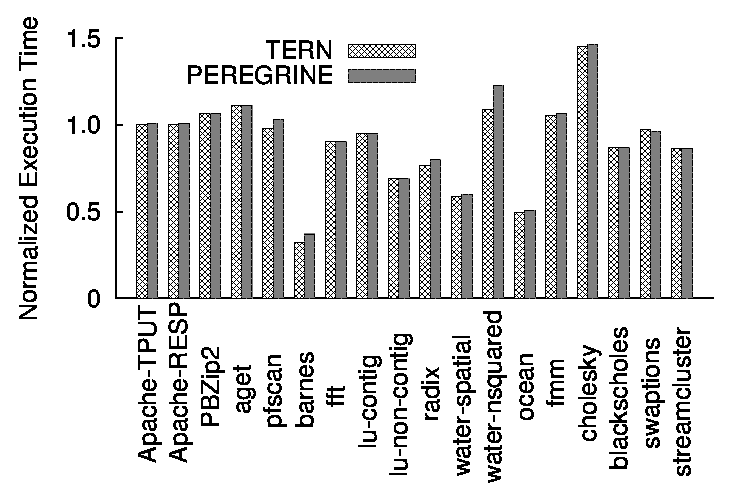
\includegraphics[width=.8\columnwidth]{tern/figures/overhead}
\vspace{-.3in}
\caption{{\em Relative overhead when reusing schedules.} } \label{fig:tern-overhead}
\vspace{-.05in}
\end{figure}


\subsubsection{Efficiency} \label{sec:tern-efficient}

Figure~\ref{fig:overhead} shows the relative overhead of \tern over
nondeterministic execution when reusing schedules, the smaller the better.  For seven out of
the fourteen programs, the replayer performed almost identically to
nondeterministic execution. For \pbzip and barnes, \tern performed
better.  This speedup came partially from the optimization to remove
unnecessary synchronizations~\cite{cui:tern:osdi10}.  \tern's overhead
for MySQL, volrend, raytrace, water-nsquared, and choleskey is relatively
large because these programs performed many synchronization operations
over a short period of time.  For instance, water-nsquared and cholesky
both call \v{pthread\_mutex\_lock()} and \v{pthread\_mutex\_unlock()} in a
tight loop.






%% Macros.
\newcommand{\bddbddb}{\vv{bddbddb}\xspace}
\newcommand{\peregrinenprog}[0]{18\xspace}

\chapter{Efficiently Enforcing Schedules without Deviation} \label{sec:peregrine}

The last chapter presents \tern, the first multithreading system that is both 
stable and deterministic. However, \tern enforces best-effort determinism, and 
its executions may deviate from the memoized schedules when data races exist. 
Thus, a second challenge on building \smt arises: how to efficiently make 
executions follow schedules and do not deviate? This challenge also exists in 
the area of deterministic execution and replay for decades. To address this 
challenge, this chapter presents \peregrine, our second \smt (and also \dmt) 
with a new technique called \emph{schedule relaxation}.

\section{Introduction} \label{sec:peregrine-intro}

%% Why multithreading is so difficult to get right. Too many schedules.
%% All inputs, each input (define nondeterminism). Must refer to Chapter 2:
%% motivation.
As described in Chapter~\ref{sec:smt-motivation}, a root cause that makes 
multithreaded programs so difficult to get right is: these
programs have exponentially many possible schedules for all inputs at
runtime. Even running on the same input, the concurrently running threads of a
program may interleave in too many different ways, depending on such factors as
hardware timing and OS scheduling. This is the so called ``nondeterminism."
Considering all inputs, the number of possible schedules is even greater. It is
extremely challenging to understand, test, analyze, or verify all
these schedules in a multithreaded program. Therefore, a concurrency bug within
an unchecked schedule can show up in production runs and lead to severe
failures and vulnerabilities.

To reduce the number of possible schedules and make multithreading easier to get
right, two complementary techniques have been invented by researchers recently.
\smt~\cite{determinator:osdi10, cui:tern:osdi10}, 
which is created by my collaborators and me, aims to reduce the number possibles
schedules on all inputs. 
\dmt~\cite{dmp:asplos09,kendo:asplos09,coredet:asplos10,
dos:osdi10,grace:oopsla09} addresses the nondeterminism problem, and it focuses
on reducing the number of possible schedules on each input down to one. Notably,
our \tern system described in Chapter~\ref{sec:tern} is the first 
multithreading system that is both stable and deterministic. Unfortunately, 
despite these effort, an open challenge~\cite{wodet11}
well recognized by the research community remains: how to build \emph{both
deterministic and efficient} \dmt systems for general multithreaded programs on
commodity multiprocessors.  Existing \dmt systems either incur prohibitive
overhead, or are not fully deterministic if there are data races.

%% Why hard. Introduce two forms of schedules
%%(1) sync schedule can be made efficient, but not fully determnistic.
%%(2) Mem schedule can be made fully determinsitic, but not efficient.

%% Our core technique. Schedule relaxation.
%%And why it can be stable, deterministic, and efficient.


% Different runs of a multithreaded program may show different behaviors,
% depending on how the threads interleave.  This \emph{nondeterminism} makes
% it difficult to write, test, and debug multithreaded programs.  For
% instance, testing becomes less assuring because the schedules tested may
% not be the ones run in the field.  Similarly, debugging can be a nightmare
% because developers may have to reproduce the exact buggy schedules.  These
% difficulties have resulted in many ``heisenbugs'' in widespread
% multithreaded programs~\cite{lu:concurrency-bugs}.

% Recently, researchers have pioneered a technique called
% \emph{Deterministic Multithreading (\dmt)}
% \cite{cui:tern:osdi10,dmp:asplos09,kendo:asplos09,coredet:asplos10,
% dos:osdi10,grace:oopsla09}.
% DMT systems ensure that the same input
% is always processed with the same deterministic schedule, thus eliminating
% heisenbugs and problems due to nondeterminism.  Unfortunately,
% despite these efforts, an open challenge~\cite{wodet11} well recognized by
% the DMT community remains: how to build \emph{both deterministic
%   and efficient} DMT systems for general multithreaded programs on
% commodity multiprocessors.  Existing DMT systems either incur prohibitive
% overhead, or are not fully deterministic if there are data races.

Specifically, existing DMT systems enforce two forms of schedules: (1) a
\emph{mem-schedule} is a deterministic schedule of shared memory
accesses~\cite{dmp:asplos09,coredet:asplos10,dos:osdi10}, such as
\vv{load/store} instructions, and (2) a \emph{sync-schedule} is a
deterministic order of synchronization
operations~\cite{kendo:asplos09,cui:tern:osdi10}, such as
\vv{lock()/unlock()}.  Enforcing a mem-schedule is truly deterministic even
for programs with data races, but may incur prohibitive overhead (\eg,
roughly 1.2\X-6\X~\cite{coredet:asplos10}).  Enforcing a sync-schedule is
efficient (\eg, average 16\% slowdown~\cite{kendo:asplos09}) because
most code does not control synchronization and can still run in
parallel, but a sync-schedule is only deterministic for race-free
programs, when, in fact, most real programs have races, harmful or
benign~\cite{lu:concurrency-bugs,syncfinder:osdi10}.  The dilemma is,
then, to pick either determinism or efficiency but not both.

Our key insight is that although most programs have races, these races
tend to occur only within minor portions of an execution, and the majority
of the execution is still race-free.  Thus, we can resort to a
mem-schedule only for the ``racy'' portions of an execution and enforce a
sync-schedule otherwise, combining both the efficiency of sync-schedules
and the determinism of mem-schedules. We call these combined schedules
\emph{hybrid schedules}.

Based on this insight, we have built \peregrine, an efficient \dmt
system to address the aforementioned open challenge.
When a program first runs on an input, \peregrine records a detailed execution
trace including memory accesses in case the execution runs into races.
\peregrine then \emph{relaxes} this detailed trace into a hybrid schedule,
including (1) a total order of synchronization operations and (2) a set of
execution order constraints to deterministically resolve each occurred race. 
When the same input is provided again, \peregrine can reuse this schedule
deterministically and efficiently.

Reusing a schedule only when the program input matches exactly is too
limiting, and we aim to make \peregrine also a \smt system that can frequently
reuse schedules on a wide range of inputs.  Fortunately, the schedules
\peregrine computes are often
``coarse-grained" and reusable on a broad range of inputs.  Indeed, our
previous work has shown that a small number of sync-schedules can often cover
over 90\% of the workloads for real programs such as
\apache~\cite{cui:tern:osdi10}.  The higher the reuse rates, the more efficient
\peregrine is.

% Moreover, by reusing schedules, \peregrine makes program
% behaviors more \emph{stable} across different inputs, so that slight input
% changes do not lead to vastly different schedules~\cite{cui:tern:osdi10} and
% thus ``\emph{input-heisenbugs}" where slight input changes cause concurrency
% bugs to appear or disappear.

Before reusing a schedule on an input, \peregrine must check that the input
satisfies the input constraints of the schedule, so
that (1) the schedule is feasible, \ie, the execution on the input will reach
all events in the same deterministic order as in the schedule and (2) the
execution will not introduce new races. (New races may occur if they are
\emph{input-dependent}; see \S\ref{sec:peregrine-interthread-slice}.)  A na\"ive
approach is to collect preconditions from all input-dependent branches in
an execution trace.  For instance, if a branch instruction inspects
input variable \vv{X} and goes down the true branch, we collect a
precondition that \vv{X} must be nonzero.  Preconditions collected via
this approach ensures that an execution on an input satisfying the
preconditions will always follow the path of the recorded execution in all
threads.  However, many of these branches concern thread-local
computations and do not affect the program's ability to follow the
schedule. Including them in the preconditions thus unnecessarily decreases
schedule-reuse rates.

How can \peregrine compute sufficient preconditions to avoid new races and
ensure that a schedule is feasible?  How can \peregrine filter out unnecessary
branches to increase schedule-reuse rates?  Our previous
work, \tern~\cite{cui:tern:osdi10}, requires developers to grovel through the
code and mark the input affecting schedules; even so, it does not
guarantee full determinism if there are data races.

\peregrine addresses these challenges with two new
program analysis techniques.  First, given an execution trace and a hybrid
schedule, it computes sufficient preconditions using
\emph{determinism-preserving slicing}, a new precondition
slicing~\cite{castro:bouncer} technique designed for multithreaded
programs.  Precondition slicing takes an execution trace and a
\emph{target} instruction in the trace, and computes 
a \emph{trace slice} that captures the instructions required for the
execution to reach the target with equivalent operand
values.  Intuitively, these instructions include ``branches whose
  outcome matters" to reach the target and ``mutations that affect the
  outcome of those branches"~\cite{castro:bouncer}.  This trace slice
typically has much fewer branches than the original execution trace,
so that we can compute more relaxed preconditions.  However, previous
work~\cite{castro:bouncer} does not compute correct trace slices for
multithreaded programs or handle multiple targets; our slicing
technique correctly handles both cases.

Our slicing technique often needs to determine whether two pointer
variables may point to the same object.  \emph{Alias
  analysis} is the standard static technique to answer these queries.
Unfortunately, one of the best alias analyses~\cite{bddalias:pldi04} yields
overly
imprecise results for 30\% of the evaluated programs, forcing \peregrine to
reuse
schedules only when the input matches almost exactly.  The reason is that
standard
alias analysis has to be conservative and assume all possible executions,
yet \peregrine cares about alias results
according only to the executions that reuse a specific schedule.  To
improve precision, \peregrine uses \emph{schedule-guided simplification} to
first simplify a program according to a schedule, then runs standard alias
analysis on the simplified program to get more precise results.  For
instance, if the schedule dictates eight threads, \peregrine can clone
the corresponding thread function eight times, so that alias analysis can
separate the results for each thread, instead of imprecisely merging
results for all threads.

We have built a prototype of \peregrine that runs in user-space.
It automatically tracks \vv{main()}
arguments, data read from files and sockets, and values
returned by \vv{random()}-variants as input.  It handles long-running servers by
splitting their executions into \emph{windows} and
reusing schedules across windows~\cite{cui:tern:osdi10}.
The hybrid schedules it computes are fully deterministic for programs that
(1) have no nondeterminism sources beyond thread scheduling, data races, and
inputs tracked by \peregrine and (2) adhere to the assumptions of the tools
\peregrine uses.

We evaluated \peregrine on a diverse set of \peregrinenprog programs, including
the
\apache web server~\cite{apache}; three desktop programs, such as
\pbzip~\cite{pbzip2}, a parallel compression utility; implementations of
12 computation-intensive algorithms in the popular \splash and \parsec
benchmark suites; and \racey~\cite{racy-stress}, a benchmark with numerous
intentional races for evaluating deterministic execution and replay
systems.  Our results show that \peregrine is both deterministic and efficient
(executions reusing schedules range from 68.7\% faster to 46.6\% slower
than nondeterministic executions); it can frequently reuse schedules for
half of the programs (\eg, two schedules cover all possible inputs to
\pbzip compression as long as the number of threads is the same); both its
slicing and
simplification techniques are crucial for increasing schedule-reuse rates,
and have reasonable overhead when run offline; its recording overhead
is relatively high, but can be reduced using existing
techniques~\cite{idna:vee06}; and it requires no manual effort except a
few annotations for handling server programs and for improving precision.

Our main contributions are the schedule-relaxation approach and \peregrine, an
 efficient stable and deterministic multithreading system.  Additional 
contributions include
the ideas of hybrid schedules, determinism-preserving slicing, and
schedule-guided simplification.  To our knowledge, our slicing technique
is the first to compute correct (non-trivial) preconditions for
multithreaded programs.
We believe these ideas apply beyond \peregrine (\S\ref{sec:peregrine-deploy}).

The remainder of this chapter is organized as follows.  We first present a
high-level design of \peregrine (\S\ref{sec:peregrine-design}).  We then
describe its
core ideas: hybrid schedules (\S\ref{sec:peregrine-schedule}),
determinism-preserving slicing (\S\ref{sec:peregrine-slice}), and
schedule-guided
simplification (\S\ref{sec:peregrine-guide}).  We then present implementation
issues
(\S\ref{sec:peregrine-impl}) and evaluation (\S\ref{sec:peregrine-eval}).  We
finally discuss
related work (\S\ref{sec:peregrine-related}) and conclude
(\S\ref{sec:peregrine-summary}).

\section{High-Level Design} \label{sec:peregrine-design}

\begin{figure}[t]
\centering
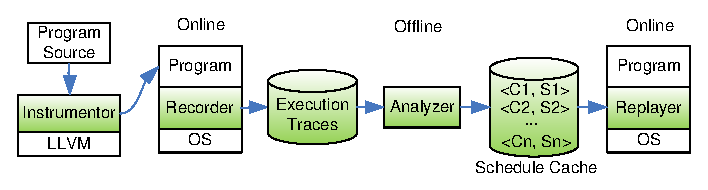
\includegraphics[width=.96\columnwidth]{peregrine/figures/overview.eps}
\caption{{\em \peregrine Architecture: components and data structures are
    shaded (and in green).}}\label{fig:peregrine-arch}
\end{figure}


Figure~\ref{fig:peregrine-arch} shows the architecture of \peregrine.  It has four main
components: the instrumentor, recorder, analyzer, and
replayer.  The \emph{instrumentor} is an LLVM~\cite{llvm} compiler plugin
that prepares a program for use with \peregrine.  It instruments synchronization
operations such as \vv{pthread\_mutex\_lock()}, which the recorder and
replayer control at runtime.  It marks the \vv{main()} arguments, data read
from \vv{read()}, \vv{fscanf()}, and \vv{recv()}, and values
returned by \vv{random()}-variants as
inputs.  We chose LLVM~\cite{llvm} as our instrumentation framework for
its compatibility with GCC and easy-to-analyze intermediate representation
(IR).  However, our approach is general and should apply beyond LLVM.
For clarity, we will present our examples and algorithms at the
source level, instead of the LLVM IR level.

The \emph{recorder} is similar to existing systems that deterministically
record executions~\cite{scribe:sigmetrics10,idna:vee06,smp-revirt:vee08}.
Our current recorder is implemented as an LLVM interpreter.  When a
program runs, the recorder saves the LLVM instructions interpreted for
each thread into a central log file.  The recorder does not record
external input data, such as data read from a file, because our
analysis does not need this information.  To schedule synchronization
operations issued by different threads, the recorder can use a variety of
DMT algorithms~\cite{cui:tern:osdi10}.  


\begin{figure}
\centering
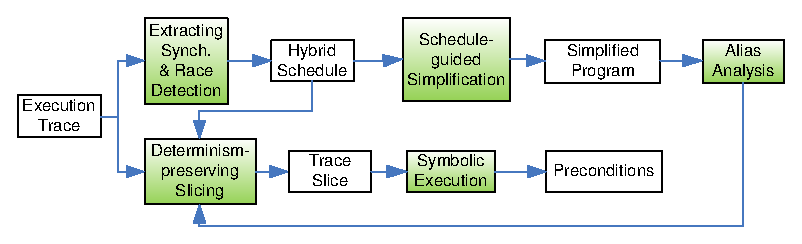
\includegraphics[width=\columnwidth]{peregrine/figures/analyzer.eps}
\caption{{\em Analyses performed by the analyzer.}}\label{fig:peregrine-analyzer}
\end{figure}

The \emph{analyzer} is a stand-alone program that computes (1) a hybrid
schedule $S$ and (2) the preconditions $C$ required for reusing the schedule on
future inputs.  It does so using a series of analyses, shown in
Figure~\ref{fig:peregrine-analyzer}.  To compute a hybrid schedule, the analyzer
first extracts a total order of synchronization operations from the
execution trace.  It then detects data races according to this
synchronization order, and computes additional \emph{execution order} constraints
to deterministically resolve the detected races.
To compute the preconditions of a schedule, the analyzer first
\emph{simplifies} the program according to the schedule, so that alias
analysis can compute more precise results.  
It then slices the execution trace into a trace slice with instructions
required to avoid new races and reach all events in the schedule.  It
then uses \emph{symbolic execution}~\cite{symbolic-execution} to
collect preconditions from the input-dependent branches in the slice.
The trace slice is typically much smaller than the execution trace, so
that the analyzer can compute relaxed preconditions, allowing frequent
reuses of the schedule.  The analyzer finally stores $\langle C, S
\rangle$ into the schedule cache, which conceptually holds a set of such
tuples. (The actual representation is tree-based for fast
lookup~\cite{cui:tern:osdi10}.)



The \emph{replayer} is a lightweight user-space scheduler for reusing
schedules.  When an input arrives, it searches the schedule cache for a
$\langle C, S \rangle$ tuple such that the input satisfies the
preconditions $C$.  If it finds such a tuple, it simply runs the program
enforcing schedule $S$ efficiently and deterministically.  Otherwise,
it forwards the input to the recorder.
%  to record an execution and compute a new $\langle C, S \rangle$ tuple.

In the remainder of this section, we first use an example to illustrate
how \peregrine works, highlighting the operation of the analyzer
(\S\ref{sec:peregrine-example}).  We then describe \peregrine's deployment and usage
scenarios (\S\ref{sec:peregrine-deploy}) and assumptions (\S\ref{sec:peregrine-limitations}).

\subsection{An Example} \label{sec:peregrine-example}

%% \begin{figure}[t]
%% %\centering
%% \hspace{-.25in}
%% \begin{minipage}[t]{.525\textwidth}
%% \centering
%% 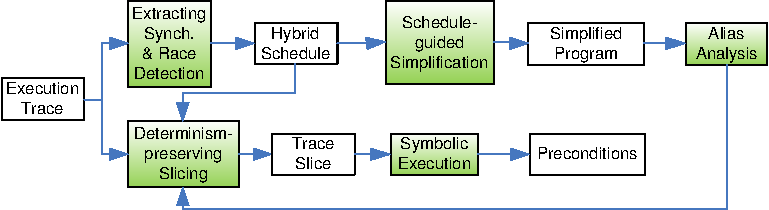
\includegraphics[width=\textwidth]{figures/analyzer}
%% \end{minipage}
%% \caption{{\em Analysis performed by the analyzer.}}\label{fig:analyzer}
%% \end{figure}

\begin{figure}[t]
\centering
\begin{minipage}{.5\textwidth}
\lgrindfile{peregrine/code/example.cpp.tex}
\end{minipage}
\caption{{\em Running example.} It uses the common
  divide-and-conquer idiom to split work among multiple threads.
  It contains write-write (lines L8 and L15)
  and read-write (lines L9 and L15) races on \vv{result} because
  of missing \vv{pthread\_join()}.} \label{fig:peregrine-example}
\end{figure}

Figure~\ref{fig:peregrine-example} shows our running example, a simple multithreaded
program based on the real ones used in our evaluation.  It first parses
the command line arguments into \vv{nthread} (line L1) and \vv{size} (L2),
then spawns \vv{nthread} threads including the main thread (L4--L5) and
processes \vv{size/nthread} bytes of data in each thread.  The thread
function \vv{worker()} allocates a local buffer (L10), reads data from a
file (L11), processes the data (L12--L13), and sums the results into
the shared variable \vv{result} (L14--L16).  The \vv{main()} function may
further update \vv{result} depending on \vv{argv[3]} (L7--L8), and finally
prints out \vv{result} (L9).  This example has read-write and write-write
races on \vv{result} due to missing \vv{pthread\_join()}.  This error
pattern matches some of the real errors in the evaluated programs such as
\pbzip.

\para{Instrumentor.} To run this
program with \peregrine, we first compile it into LLVM IR and instrument it with
the instrumentor.  The instrumentor replaces the synchronization
operations (lines L5, L14, and L16) with \peregrine-provided wrappers controlled by
the recorder and replayer at runtime.  It also inserts code to mark 
the contents of \vv{argv[i]} and the data from \vv{read()} (line L11) as
input.

\begin{figure}[t]
\begin{minipage}[t]{\columnwidth}
\centering
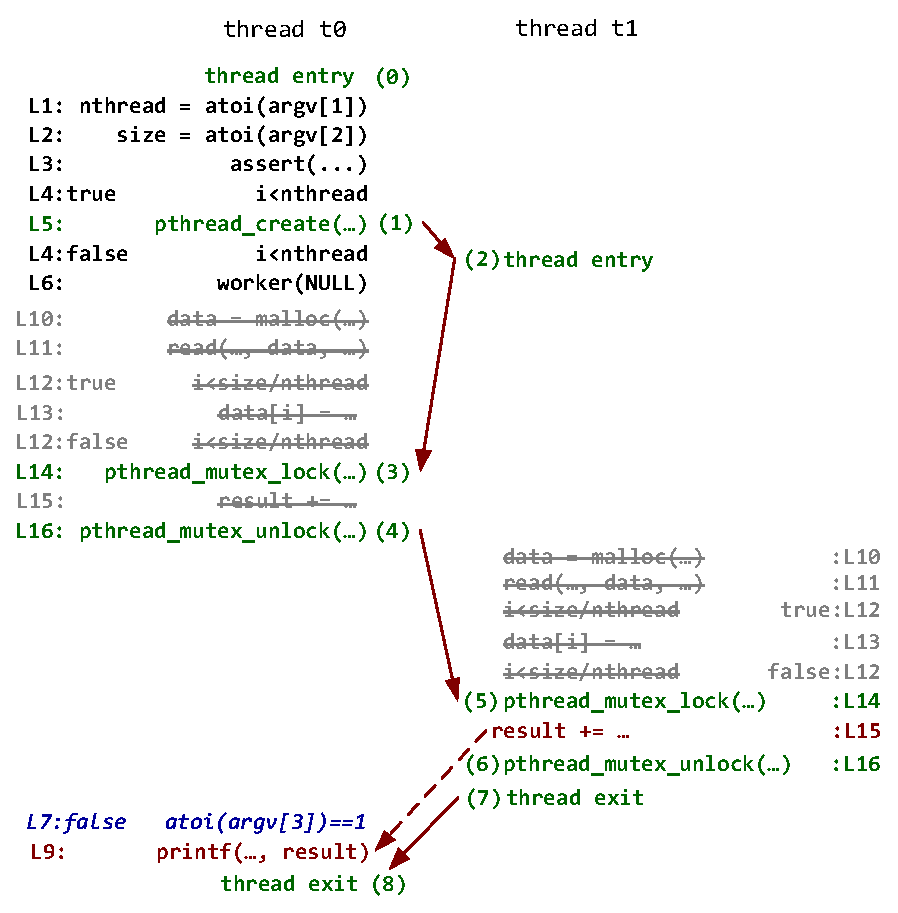
\includegraphics[width=\textwidth]{peregrine/figures/trace}
\end{minipage}
\caption{{\em Execution trace, hybrid schedule, and trace slice.}  An
  execution trace of the program in Figure~\ref{fig:peregrine-example} on arguments
  ``\vv{2 2 0}'' is shown.  Each executed instruction is tagged
  with its static line number L$i$.  Branch instructions are also tagged
  with their outcome (true or false).  Synchronization operations (green),
  including thread entry and exit, are tagged
  with their relative positions in the synchronization order.  They form a
  sync-schedule whose order constraints are shown with solid arrows.  L15 of
  thread $t_1$ and L9 of thread $t_0$ race on \vv{result}, and this race is
  deterministically resolved by enforcing an execution order constraint
  shown by the dotted arrow.  Together, these order constraints form a hybrid
  schedule.  Instruction L7 of $t_0$ (italic and blue) is included in the
  trace slice to avoid new races, while L6, L4:false, L4:true, L3, L2, and
  L1 of $t_0$ are included due to intra-thread
  dependencies. Crossed-out (gray) instructions are elided from the
  slice.}\label{fig:peregrine-trace}
\end{figure}

\para{Recorder: execution trace.}
When we run the instrumented program with arguments ``\vv{2 2 0}'' to spawn
two threads and process two bytes of data, suppose that the recorder records
the execution trace in Figure~\ref{fig:peregrine-trace}.  (This figure also shows
the hybrid schedule and preconditions \peregrine computes, explained
later in this subsection.)  This trace is just one
possible trace depending on the scheduling algorithm the recorder uses.

\para{Analyzer: hybrid schedule.}
Given the execution trace, the analyzer starts by computing a hybrid
schedule.  It first extracts a sync-schedule consisting of the operations
tagged with (1), (2), ..., (8) in Figure~\ref{fig:peregrine-trace}.  It then detects races in
the trace according to this sync-schedule, and finds the race on
\vv{result} between L15 of thread $t_1$ and L9 of $t_0$.  It then computes an
execution order constraint to deterministically resolve this race, shown
as the dotted arrow in Figure~\ref{fig:peregrine-trace}.  The sync-schedule and
execution order constraint together form the hybrid schedule.  Although
this hybrid schedule constrains the order of synchronization and the last
two accesses to \vv{result}, it can still be efficiently reused because the
core computation done by \vv{worker} can still run in parallel.


\para{Analyzer: simplified program.}
To improve analysis precision, the analyzer simplifies the program according to the
hybrid schedule.  For instance, based on the number of
\vv{pthread\_create()} operations in the schedule, the analyzer
clones function \vv{worker()} to give each thread a copy,
so that the alias analysis separates different threads and determines that
the two instances of L13 in $t_0$ and $t_1$ access different
\vv{malloc}'ed locations and never race.

\para{Analyzer: trace slice.}
The analyzer uses
determinism-preserving slicing to reduce the execution trace into a trace
slice, so that it can compute relaxed preconditions.
The final trace slice consists of the instructions not crossed out
in Figure~\ref{fig:peregrine-trace}.
The analyzer computes this trace slice using inter-thread and 
intra-thread steps.  In the inter-thread step, it adds instructions
required to avoid new races into the slice.  Specifically, for $t_0$ it adds
the false branch of L7, or L7:false, because if the true branch
is taken, a new race between L8 of $t_0$ and L15 of $t_1$ occurs.  It
ignores branches of line L12 because alias analysis already determines that L13 of
$t_0$ and L13 of $t_1$ never race.

In the intra-thread step, the analyzer adds instructions required 
to reach all instructions identified in the
inter-thread step (L7:false of $t_0$ in this example) and all events in
the hybrid schedule.  It does so by traversing the execution trace
backwards and tracking control- and data-dependencies.  In this example, it
removes L15, L13, L12, L11, and L10 because no instructions currently in
the trace slice depend on them.  It adds L6 because without this call, the
execution will not reach instructions L14 and L16 of thread $t_0$.  It adds
L4:false because if the true branch is taken, the execution of $t_0$ will
reach one more \vv{pthread\_create()}, instead of L14,
\vv{pthread\_mutex\_lock()}, of $t_0$.  It adds L4:true because this branch
is required to reach L5, the \vv{pthread\_create()} call.  It similarly
adds L3, L2, and L1 because later instructions in the trace slice
depend on them.


\para{Analyzer: preconditions.}
After slicing, all branches from L12 are gone.  The
analyzer joins the remaining branches together as the
preconditions, using a version of \klee~\cite{klee:osdi08} augmented with
thread support~\cite{cui:tern:osdi10}.  Specifically, the analyzer marks
input data as \emph{symbolic}, and then uses \klee to track how this symbolic
data is propagated and observed by the instructions in the trace slice.
(Our \peregrine prototype runs symbolic execution within the recorder for
simplicity; see \S\ref{sec:peregrine-record}.)
If a branch instruction inspects symbolic data and proceeds down the true
branch, the analyzer adds the precondition that the symbolic data makes
the branch condition true.  The analyzer uses symbolic
summaries~\cite{castro:bouncer} to succinctly generalize common library
functions.  For instance, it considers the return of \vv{atoi(arg)}
symbolic if \vv{arg} is symbolic.

\begin{figure}[t]
\centering
\begin{minipage}[t]{3.1in}
\begin{scriptsize}
$(atoi\_argv_1 = 2) \wedge (atoi\_argv_2 \geq atoi\_argv_1) \wedge
  (atoi\_argv_3 \neq 1) $
\end{scriptsize}
\end{minipage}
\caption{{\em Preconditions computed from the trace slice in
    Figure~\ref{fig:peregrine-trace}.}  Variable $atoi\_argv_i$ represents the
  return of \vv{atoi(arg[i])}.} \label{fig:peregrine-precond}
\end{figure}

Figure~\ref{fig:peregrine-precond} shows the preconditions the analyzer computes
from the trace slice in Figure~\ref{fig:peregrine-trace}.
These preconditions illustrate two key benefits of \peregrine.
First, they are sufficient to ensure deterministic reuses of the schedule.
Second, they only loosely constrain the data size ($atoi\_argv_2$) and do
not constrain the data contents (from \vv{read()}), allowing frequent
schedule-reuses.  The reason is that L10--L13 are all sliced out.
One way to leverage this benefit is to populate a
schedule cache with small workloads to reduce analysis time, and then
reuse the schedules on large workloads.

\para{Replayer.}
Suppose we run this program again on different arguments ``\vv{2 1000 8}.''
The replayer checks the new arguments against the preconditions in
Figure~\ref{fig:peregrine-precond} using \klee's constraint checker, and finds that these
arguments satisfy the preconditions, despite the much larger data size.  
It can therefore reuse the hybrid schedule in Figure~\ref{fig:peregrine-trace}
on this new input by enforcing
the same order of synchronization operations and accesses
to \vv{result}.


\subsection{Deployment and Usage Scenarios} \label{sec:peregrine-deploy}

\peregrine runs in user-space and requires no special hardware, presenting few
challenges for deployment.  To populate a schedule cache, a user can
record execution traces from real workloads;
or a developer can run (small) representative workloads
to pre-compute schedules before deployment.  \peregrine
efficiently makes the behaviors of multithreaded programs more repeatable,
even across a range of inputs.  We envision that users can use this repeatability in
at least four ways.

\para{Concurrency error avoidance.} \peregrine can reuse well-tested schedules
collected from the testing lab or the field, reducing the risk of running
into untested, buggy schedules.  
Currently \peregrine detects and avoids only data races.  However, combined with
the right error detectors, \peregrine can be easily extended to detect and
avoid other types of concurrency errors.

\para{Record and replay.} Existing deterministic record-replay systems
tend to incur high CPU and storage overhead (\eg, 15X
slowdown~\cite{idna:vee06} and 11.7 GB/day
storage~\cite{smp-revirt:vee08}).  A record-replay system on top of \peregrine
may drastically reduce this overhead: for inputs that hit the
schedule cache, we do not have to
log any schedule.

\para{Replication.}
To keep replicas of a multithreaded program consistent, a replication tool
often records the thread schedules at one replica and replays them at
others.  This technique is essentially \emph{online}
replay~\cite{respec:asplos10}.
It may thus incur high CPU, storage, and
bandwidth overhead.  With \peregrine, replicas can maintain a consistent
schedule cache.  If an input hits the schedule cache, all replicas will
automatically select the same deterministic schedule, incurring zero
bandwidth overhead.

\para{Schedule-diversification.}  Replication can tolerate
hardware or network failures, but the replicas may still run into the same
concurrency error because they all use the same schedules.  Fortunately,
many programs are already ``mostly-deterministic'' as they either compute
the same correct result or encounter heisenbugs.  We can thus run \peregrine to
deterministically diversify the schedules at different replicas (\eg,
using different scheduling algorithms or schedule caches) to tolerate
\emph{unknown} concurrency errors.

\para{Applications of individual techniques.} The individual ideas in \peregrine
can also benefit other research efforts.  For instance, hybrid schedules
can make the sync-schedule approach deterministic without recording
executions, by coupling it with a sound static race detector.
Determinism-preserving slicing can (1) compute input filters to block bad
inputs~\cite{castro:bouncer} causing concurrency errors and (2) randomize
an input causing a concurrency error for use with anonymous bug
reporting~\cite{castro:bug-report-privacy}.  Schedule-guided
simplification can transparently improve the precision of many existing
static analyses: simply run them on the simplified programs.  This improved
precision may be leveraged to accurately detect errors or even
verify the correctness of a program according to a set of schedules.
Indeed, from a verification perspective, our simplification technique
helps \emph{verify} that executions reusing schedules have \emph{no}
new races.


\subsection{Assumptions} \label{sec:peregrine-limitations}

At a design level, we anticipate the schedule-relaxation approach to work
well for many programs/workloads as long as (1) they can benefit from
repeatability, (2) their schedules can be frequently reused, (3) their
races are rare, and (4) their nondeterminism comes from the sources
tracked by \peregrine.  This approach is certainly not designed for every
multithreaded program. For instance, like other DMT systems, \peregrine should
not be used for parallel simulators that desire nondeterminism for
statistical confidence.  For programs/workloads that rarely reuse
schedules, \peregrine may be unable to amortize the cost of recording and
analyzing execution traces.  For programs full of races, enforcing hybrid
schedules may be as slow as mem-schedules.  \peregrine addresses nondeterminism
due to thread scheduling and data races.  It mitigates input
nondeterminism by reusing schedules on different inputs.  It currently
considers command line arguments, data read from a file or a socket, and
the values returned by \v{random()}-variants as inputs.  \peregrine ensures that
schedule-reuses are fully deterministic if a program contains only these
nondeterminism sources, an assumption met by typical programs.  If a
program is nondeterministic due to other sources, such as functions that
query physical time (\eg, \v{gettimeofday()}), pointer addresses returned
by \v{malloc()}, and nondeterminism in the kernel or external libraries,
\peregrine relies on developers to annotate these sources.


%\peregrine leverages a set of techniques such as symbolic execution, program
% slicing, and alias analysis.  
The underlying techniques that \peregrine leverages make assumptions as well.
\peregrine computes preconditions from a trace slice using the symbolic
execution engine \klee, which does not handle floating point operations;
though recent work~\cite{klee-fp} has made advances in symbolic execution
of floating point programs.  (Note
that floating point operations not in trace slices are not an issue.)  We
explicitly designed \peregrine's slicing technique to compute sufficient
preconditions, but these preconditions may still include unnecessary ones,
because computing the \emph{weakest} (most relaxed) preconditions in general is
undecidable~\cite{aho:dragon:06}.  The alias analysis \peregrine uses makes a
few assumptions about the analyzed programs~\cite{alias:icse05};
a ``sounder'' alias analysis~\cite{alias:fse06} would remove these
assumptions.  These analyses may all get expensive for large
programs.  For server programs, \peregrine borrows the
windowing idea from our previous work~\cite{cui:tern:osdi10}; it is thus
similarly limited (\S\ref{sec:peregrine-window}).

At an implementation level, \peregrine uses the LLVM framework, thus requiring
that a program is in either source (so we can compile using LLVM) or LLVM
IR format.  \peregrine ignores inline x86 assembly or calls to external
functions it does not know.  For soundness, developers have to lift x86
assembly to LLVM IR and provide summaries for external functions.  (The
external function problem is alleviated because \klee comes with a
\v{Libc} implementation.)  Currently \peregrine works only with a single process,
but previous work~\cite{dos:osdi10} has demonstrated how \dmt systems can
be extended to multiple processes.

%The preconditions \peregrine computes are not the \emph{weakest
%  preconditions}~\cite{aho:dragon:06} (\ie, most relaxed preconditions),


%relies on developers to annotate the boundaries of request processing and
%the functions that observe the internal state of the servers.

%% For instance, a parallel quick sort program may rarely reuse schedules
%% because it nondeterministically partitions data based on randomly chosen
%% pivots.  Fortunately, for performance, most parallel programs use
%% deterministic partitions of data, such as commonly used parallel sort with
%% sorting networks~\cite{sorting-networks} and 
%% all programs we have evaluated except \apache (because it does no
%% partitioning: it processes each client request with only one worker
%% thread).

% boundary: proxy process like dos

%% includes only the instructions dependent by the events
%% in the schedule.  control, data-dependency may not be widely
%% understood.  It does so by computing control- and data-dependencies,
%% within the same thread for reachability and across different threads for
%% determinism.  



\section{Hybrid Schedules} \label{sec:schedule}

This section describes how \peregrine computes (\S\ref{sec:compute-schedule})
and enforces (\S\ref{sec:enforce-schedule}) hybrid schedules.

\subsection{Computing Hybrid Schedules} \label{sec:compute-schedule}

To compute a hybrid schedule, \peregrine first extracts a total order of
synchronization operations from an execution trace.  Currently, it
%\peregrine
considers 28 \v{pthread} operations, such as \v{pthread\_mutex\_lock()}
and \v{pthread\_cond\_wait()}.  It also considers
the entry and exit of a thread as synchronization operations so that it can
order these events together with other synchronization operations.  These
operations are sufficient to run the programs evaluated, and more can be
easily added.  \peregrine uses a total, instead of a partial, order because
previous work has shown that a total order is already
efficient~\cite{cui:tern:osdi10,kendo:asplos09}.

\begin{figure}[t]
\centering
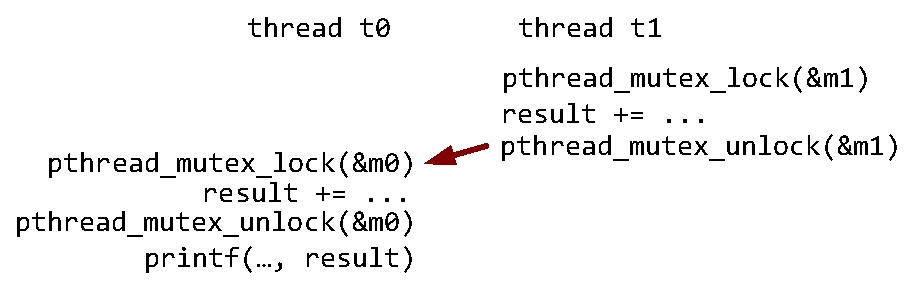
\includegraphics[width=.9\columnwidth]{peregrine/figures/concurrent-intervals.eps}
\caption{{\em No \peregrine race with respect to this
    schedule.}} \label{fig:concurrent-intervals}
\end{figure}

For determinism, \peregrine must detect races that occurred during the recorded
execution and compute execution order constraints to deterministically
resolve the races.  An off-the-shelf race detector would flag too many
races because it considers the original synchronization
constraints of the program, whereas \peregrine wants to detect races according
to a sync-schedule~\cite{pres:sosp09,recplay:tocs}.  To illustrate,
consider Figure~\ref{fig:concurrent-intervals}, a modified sync-schedule
based on the one in Figure~\ref{fig:trace}.  Suppose the two threads
acquire different mutex variables, and thread $t_1$ acquires and releases
its mutex before $t_0$.  Typical lockset-based~\cite{savage:eraser}
or happens-before-based~\cite{lamportclock} race detectors would flag a
race on \v{result}, but our race detector does not: the sync-schedule
in the figure deterministically resolves the order of accesses to \v{result}.  
Sync-schedules anecdotally reduced the number of
possible races greatly, in one extreme case, from more than a million to
four~\cite{pres:sosp09}.


%% For instance, consider the sync-schedule in
%% Figure~\ref{fig:concurrent-intervals}.  We use $T_{m,n}$ to denote the
%% region of an execution trace executed by thread $T_m$ between this
%% thread's $(n-1)^{th}$ and $n^{th}$ synchronization operation.  By
%% enforcing the sync-schedule between unrelated operations on lock \v{l1}
%% and \v{l2}, we effectively make region $T_{1,1}$ happens-before $T_{2,2}$
%% and $T_{2,1}$ happens-before $T_{1,3}$.  Thus, we do not need to detect
%% races for these regions.  Such sync-schedules can vastly reduce the number
%% of possible races, in one extreme case, from more than a million to
%% four~\cite{pres:sosp09}.

%% \peregrine constructs a happens-before graph,
%% such as the graph in Figure~\ref{fig:concurrent-intervals}, by adding a
%% directed edge for each pair of adjacent synchronization operations in a
%% sync-schedule.  It then iterates through each pair of concurrent regions
%% defined by the happens-before graph, and flags two instructions from these
%% regions respectively as a race if they access the same memory location and
%% at least one is write.

Mechanically, \peregrine detects occurred races using a happens-before-based
algorithm.  It flags two memory accesses as a race iff (1) they access the
same memory location and at least one is a \v{store} and (2) they are
\emph{concurrent}.  To determine whether two accesses are concurrent,
typical happens-before-based detectors use vector
clocks~\cite{vectorclock} to track logically when the accesses occur.
Since \peregrine already enforces a total synchronization order, it uses a
simpler and more memory-efficient logical clock representation.

Specifically, given two adjacent synchronization operations within one
thread with relative positions $m$ and $n$ in the sync-schedule, \peregrine uses $[m,n)$ as
  the logical clock of all instructions executed by the thread between the
  two synchronization operations.  For instance, in
  Figure~\ref{fig:trace}, all instructions run by thread $t_0$
  between the \v{pthread\_mutex\_unlock()} operation and the thread exit have
  clock $[4, 8)$.
%  where $4$ and $8$ are the relative positions of the    \v{pthread\_mutex\_unlock()} operation and the thread exit in the sync-schedule.
    \peregrine considers two accesses with clocks $[m_0, n_0)$
      and $[m_1, n_1)$ concurrent if the two clock ranges overlap, \ie,
        $m_0 < n_1 \wedge m_1 < n_0$.  For instance, $[4, 8)$ and $[5,
            6)$ are concurrent.

To deterministically resolve a race, \peregrine enforces an execution order
constraint $inst_1 \rightarrow inst_2$ where $inst_1$ and $inst_2$ are the
two dynamic instruction instances involved in the race.  \peregrine identifies a
dynamic instruction instance by $\langle sid, tid, nbr \rangle$ where
$sid$ refers to the unique ID of a static instruction in the executable
file; $tid$ refers to the internal thread ID maintained by \peregrine, which
always starts from zero and increments deterministically upon each
\v{pthread\_create()}; and $nbr$ refers to the number of control-transfer
instructions (branch, call, and return) locally executed within the thread
from the last synchronization to instruction $inst_i$.  For instance, \peregrine
represents the execution order constraint in
Figure~\ref{fig:trace} as $\langle L15,t_1,0\rangle \rightarrow
\langle L9,t_0,2 \rangle$, where the branch count $2$ includes the return
from \v{worker} and the branch L7 of thread $t_0$.
We must distinguish different dynamic instances of a static instruction
because some of these dynamic instances may be involved in races while others
are not.  We do so by counting branches because if an instruction is
executed twice, there must be a control-transfer between
the two instances~\cite{smp-revirt:vee08}.  We count branches starting from the last
synchronization operation because the partial schedule preceding this
operation is already made deterministic.


%% These branch instructions include LLVM instructions \v{br} (direct conditional
%% or unconditional branch), \v{switch}, \v{indirectbr}, \v{call}, and
%% \v{invoke} (like call instruction, but with a callee that may throw
%% exceptions).  

\begin{figure}[t]
\centering
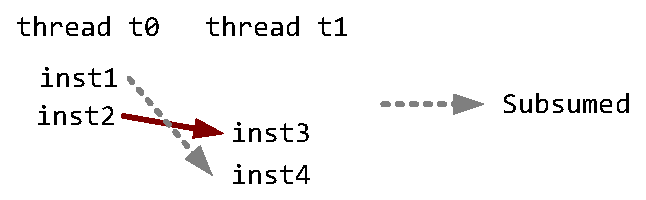
\includegraphics[width=.65\columnwidth]{peregrine/figures/pruned-order}
\caption{{\em Example subsumed execution order
    constraint.}} \label{fig:subsumed}
\end{figure}

If one execution order constraint subsumes another, \peregrine does not add the
subsumed one to the schedule.  Figure~\ref{fig:subsumed} shows a subsumed
constraint example.  Algorithmically, \peregrine considers an execution order
constraint $inst_1 \rightarrow inst_4$ subsumed by $inst_2 \rightarrow
inst_3$ if (1) $inst_1$ and $inst_2$ have the same logical clock (so they
must be executed by the same thread) and $inst_2$ occurs no earlier than
$inst_1$ in the recorded execution trace; (2) $inst_3$ and $inst_4$ have
the same logical clock and $inst_3$ occurs no later than $inst_4$ in the
trace.  This algorithm ignores
%considers only direct order constraints and 
transitive order constraints, so it may miss some subsumed constraints.
For instance, it does not consider $inst_1 \rightarrow inst_4$ subsumed if
we replace constraint $inst_2 \rightarrow inst_3$ with $inst_2 \rightarrow
inst_{other}$ and $inst_{other} \rightarrow inst_3$ where $inst_{other}$
is executed by a third thread.
% and keep other things unchanged.

\subsection{Enforcing Hybrid Schedules} \label{sec:enforce-schedule}

To enforce a synchronization order, \peregrine uses a technique called
\emph{semaphore relay}~\cite{cui:tern:osdi10} that orders synchronization
operations with per-thread semaphores.
At runtime, a synchronization wrapper
(recall that \peregrine instruments synchronization operations for runtime
control) waits on the semaphore of the current thread.  Once it is woken
up, it proceeds with the actual synchronization operation, then wakes up
the next thread according to the synchronization order.  
% Compared to an approach using locks or condition variables, semaphore
% relay avoids unnecessary lock contentions.
For programs that frequently do synchronization operations, the overhead
of semaphore may be large because it may cause a thread to block.  Thus,
\peregrine also provides a spin-wait version of
semaphore relay called \emph{flag relay}.
%% Specifically, a synchronization wrapper spin-waits on a
%% cache-aligned integer flag dedicated for the current thread, and sets the
%% flag for the next thread when its done.  Flag relay 
This technique turns out to be very
fast for many programs evaluated (\S\ref{sec:efficient}).

%% For an execution order constraint, \peregrine uses a more involved method
%% because one static instruction may have many dynamic instances.  Recall
%% that an execution order constraint has the form $inst_1 \rightarrow
%% inst_2$ where $inst_i$ are the two dynamic instruction instances
%% identified by thread ID, branch count, and static instruction ID
%% (\S\ref{sec:schedule}).  Thread ID is a deterministic thread ID maintained
%% by \peregrine.  Branch count counts locally within the thread the number of
%% branch instructions from the last synchronization operation to $inst_i$.  

% if we have space, include the slot function.

To enforce an execution order constraint, \peregrine uses program
instrumentation, avoiding the need for special hardware, such as the often
imprecise hardware branch counters~\cite{smp-revirt:vee08}.
% a more involved method to ensure that the order constraint is enforced
% on the right dynamic instance of a static instruction.
Specifically, given a dynamic instruction instance $\langle sid, tid, nbr \rangle$, \peregrine
instruments the static instruction $sid$ with a semaphore \v{up()} or
\v{down()} operation. 
%(It cannot use mutex operations because it has to deterministically
%resolve the race.)
It also instruments the branch instructions counted in $nbr$ so that when
each of these branch instructions runs, a per-thread branch counter is
incremented.  \peregrine activates the inserted semaphore operation for thread
$tid$ only when the thread's branch counter matches $nbr$.  To avoid
interference and unnecessary contention when there are multiple order
constraints, \peregrine assigns a unique semaphore to each constraint.
% To handle the special case that a semaphore operation is inserted before
% a thread does any synchronization, \peregrine considers the entry of a thread
% a synchronization operation, so that it can start branch-counting and
% activate semaphore operations from the entry of a thread.

\begin{figure}[t]
\centering
\begin{minipage}{0.45\textwidth}
\tiny \lgrindfile{peregrine/code/slot.cpp}
\end{minipage}
\vspace{-.1in}
\caption{\emph{Instrumentation to enforce execution order
    constraints.}} \label{fig:slot}
\vspace{-.1in}
\end{figure}

\peregrine instruments a program by leveraging a fast instrumentation framework we
previously built~\cite{wu:loom:osdi10}.  It keeps two versions of each
basic block: a normally compiled, fast version, and a slow backup
padded with calls to a \v{slot()} function before each instruction.  As
shown in Figure~\ref{fig:slot}, the \v{slot()} function interprets the
actions (semaphore \v{up/down}) to be taken at each instruction.  To
instrument an instruction, \peregrine simply updates the actions for that 
instruction.  This instrumentation may be expensive, but fortunately, \peregrine
leaves it off most of the time and turns it on only at the last
synchronization operation before an inserted semaphore operation.
%% instruction.  This instrumentation may be expensive, but fortunately, \peregrine
%% can leave it off most of the time: \peregrine turns it on only at the last
%% synchronization operation before an inserted semaphore operation, and
%% turns it off immediately after the inserted semaphore operation is done.

\peregrine turns on/off this instrumentation by switching a per-thread flag.
Upon each function entry, \peregrine inserts code to check this flag and
determine whether to run the normal or slow version of the basic blocks.
\peregrine also inserts this check after each function returns in case the
callee has switched the per-thread flag.  The overhead of these checks
tend to be small because the flags are rarely switched 
and hardware branch predication works well in this case~\cite{wu:loom:osdi10}.
% hardware branch predication can predicates their 

%% To turn on this instrumentation,
%%  and switches the execution to the backup by flipping a
%% per-thread switch flag.
%% \peregrine flips switch flags at the last
%% synchronization before and the first synchronization after an inserted
%% semaphore operation.  \peregrine checks switch flags to determine whether it
%% should run the fast or slow versions of a basic block at function entries
%% and call returns.

One potential issue with branch-counting is that \peregrine has to
``fix'' the partial path from the last synchronization to the dynamic
instruction instance involved in a race so that the branch-counts match
between the recorded execution and all executions
reusing the extracted hybrid schedule, potentially reducing schedule-reuse rates.
Fortunately, races are rare, so this issue has not reduced \peregrine's
schedule-reuse rates based on our evaluation.

%% from the last synchronization to the dynamic instruction instance
%% involved in an execution order constraint, the same exact branches
%% occur in the , so that


% Although a better method exists (\S\ref{sec:slice}), we have not
% implemented it because



\section{Determinism-Preserving Slicing} \label{sec:peregrine-slice}

\peregrine uses determinism-preserving slicing to (1) compute sufficient
preconditions to avoid new races and ensure that a schedule is feasible,
and (2) filter many unnecessary preconditions to increase schedule-reuse
rates.  It does so using inter- and intra-thread steps.  In the
inter-thread step (\S\ref{sec:peregrine-interthread-slice}), it detects and avoids
\emph{input-dependent} races that do not occur in the execution trace, but
may occur if we reuse the schedule on a different input.
In the intra-thread step (\S\ref{sec:peregrine-interthread-slice}), the analyzer
computes a \emph{path slice} per thread by including instructions that may
affect the events in the schedule or the instructions identified in the
inter-thread step.


\subsection{Inter-thread Step} \label{sec:peregrine-interthread-slice}

In the inter-thread step, \peregrine detects and avoids input-dependent races
with respect to a hybrid schedule.  An example input-dependent race is the
one between lines L8 and L15 in Figure~\ref{fig:peregrine-example}, which occurs when
\vv{atoi(argv[3])} returns 1 causing the true branch of L7 to be taken.
Figure~\ref{fig:peregrine-input-race-examples} shows two more types of input-dependent races.

\begin{figure}[b]
\vspace{-.1in}
\centering
\hspace{\stretch{1}}
\begin{minipage}[b]{.225\textwidth}
  \lgrindfile{peregrine/code/not-run.cpp.tex}
  \center{\vskip -3mm \hskip -5mm \scriptsize \bf (a)}
\end{minipage}
\hspace{\stretch{1}}
\begin{minipage}[b]{.225\textwidth}
  \lgrindfile{peregrine/code/br-br.cpp.tex}
  \center{\vskip -3mm \hskip -5mm \scriptsize \bf (b)}
\end{minipage}
\hspace{\stretch{1}}
\vspace{-.1in}
\caption{{\em Input-dependent races.} Race (a) occurs when
  \vv{input1} and \vv{input2} are the same; Race (b) occurs when
  both true branches are taken.} \label{fig:peregrine-input-race-examples}
\end{figure}

To detect such races, \peregrine starts by refining the logical clocks computed
based on the sync-schedule (\S\ref{sec:peregrine-compute-schedule}) with
execution order constraints because it will also enforce these
constraints.  \peregrine then iterates through all pairs
of concurrent \emph{regions}, where a region is a set of instructions with an identical
logical clock.  For each pair, it detects input-dependent races, and adds
the racy instructions to a list of \emph{slicing targets} used by the
intra-thread step.

\begin{figure}[!ht]
%%\centering
\vspace{-.3in}
\begin{minipage}[t]{\textwidth}
\tiny  \lgrindfile{peregrine/code/input-race.cpp.tex}
\end{minipage}
\vspace{-.2in}
\caption{{\em Input-dependent race detection
    algorithm.}} \label{fig:peregrine-detect-input-race}
\vspace{-.1in}
\end{figure}

Figure~\ref{fig:peregrine-detect-input-race} shows the algorithm to detect
input-dependent races for two concurrent regions.  The algorithm iterates
through each pair of instructions respectively from the
two regions, and handles three types of input-dependent races.  First, if
neither instruction is a branch instruction, it queries alias analysis to
determine whether the instructions \emph{may} race.  If so, it adds both
instructions to \vv{slicing\_targets} and adds additional
preconditions to ensure that the pointers dereferenced are different, so
that reusing the schedule on a different input does not cause the may-race
to become a real race.  Figure~\ref{fig:peregrine-input-race-examples}(a) shows
a race of this type.

Second, if exactly one of the instructions is a branch instruction, the
algorithm checks whether the instructions contained in the not-taken
branch of this instruction may race with the other instruction
(using an interprocedural \emph{post-dominator analysis}~\cite{aho:dragon:06}).
It must check the not-taken branch because a new
execution may well take the not-taken branch and cause a race.  To avoid such a
race, \peregrine adds the taken branch into the trace slice so that executions
reusing the schedule always go down the taken branch.  For instance, to
avoid the input-dependent race between lines L8 and L15
in Figure~\ref{fig:peregrine-example}, \peregrine includes
the false branch of L7 in the trace slice.

Third, if both instructions are branch instructions, the algorithm checks
whether the not-taken branches of the instructions may race, and if so, it
adds either taken branch to \vv{slicing\_targets}.
For instance, to avoid the race in Figure~\ref{fig:peregrine-input-race-examples}(b),
\peregrine includes one of the false branches in the trace slice.

For efficiency, \peregrine avoids iterating through all pairs of instructions
from two concurrent regions because instructions in one region often
repeatedly access the same memory locations.  Thus, \peregrine computes memory
locations read or written by all instructions in one region, then checks
whether instructions in the other region also read or write these memory
locations.  These locations are static operands, not dynamic
addresses~\cite{rwset:tacas08}, so that \peregrine can aggressively cache them
per static function or branch.  The complexity of our algorithm thus drops from
$O(MN)$ to $O(M+N)$ where $M$ and $N$ are the numbers of memory
instructions in the two regions respectively.


\subsection{Intra-thread Step} \label{sec:peregrine-intrathread-slice}

In the intra-thread step, \peregrine leverages a previous
algorithm~\cite{castro:bouncer} to compute a per-thread path slice,
by including instructions required for the thread to reach the
\vv{slicing\_targets} identified in the inter-thread step and the events in
the hybrid schedule.  To do so, \peregrine first prepares a per-thread ordered
target list by splitting \vv{slicing\_targets} and events in the hybrid
schedule and sorting them based on their order in the execution trace.

\peregrine then traverses the execution trace backwards to compute path slices.
When it sees a target, it adds the target to the path slice of the
corresponding thread, and starts to track the control- and
data-dependencies of this target.\footnote{For readers familiar with
  precondition slicing, \peregrine does not always track data-dependencies for
  the operands of a target.  For instance, consider instruction
  L9 of thread $t_0$ in Figure~\ref{fig:peregrine-trace}.  \peregrine's goal is
  to deterministically resolve the race involving L9 of $t_0$, but it
  allows the value of \vv{result} to be different.  Thus, \peregrine does not
  track dependencies for the value of \vv{result}, and L15 of $t_0$ is elided.}
  \peregrine adds a branch
instruction to the path slice if taking the opposite branch may cause the
thread not to reach any instruction in the current (partial) path slice;
L3 in Figure~\ref{fig:peregrine-trace} is added for this reason.
It adds a non-branch instruction to the path slice if the result of this
instruction may be used by instructions in the current path slice;
L1 in Figure~\ref{fig:peregrine-trace} is added for this reason.

A ``\vv{load p}'' instruction may depend on an earlier ``\vv{store q}'' if
\vv{p} and \vv{q} may alias even though \vv{p} and \vv{q} may not be the
same in the execution trace, because an execution on a different input
may cause \vv{p} and \v{q} to be the same.  Thus, \peregrine queries alias
analysis to compute such \emph{may}-dependencies and include the depended-upon
instructions in the trace slice.

Our main modification to~\cite{castro:bouncer} is to slice toward multiple
ordered targets.  To illustrate this need, consider branch L4:false of
$t_0$ in Figure~\ref{fig:peregrine-trace}.  \peregrine must add this branch  to thread
$t_0$'s slice, because otherwise, the thread would reach another
\vv{pthread\_create()}, a different synchronization operation than the
\vv{pthread\_mutex\_lock()} operation in the schedule.


The choice of LLVM IR has considerably simplified our slicing
implementation.  First, LLVM IR limits memory access to only two
instructions, \vv{load} and \vv{store}, so that our
algorithms need consider only these
instructions.  Second, LLVM IR uses an unlimited number of virtual registers,
so that our analysis does not get poisoned by stack spilling instructions.
Third, each virtual register is defined exactly once, and multiple
definitions to a variable are merged using a special instruction.  This
representation (\emph{static single assignment}) simplifies
control- and data-dependency tracking.  Lastly, the type information LLVM IR
preserves helps improving the precision of the alias analysis.


\section{Schedule-Guided Simplification} \label{sec:guide}

In both the inter- and intra-thread steps of determinism-preserving
slicing, \peregrine frequently queries alias analysis.  The inter-thread step
needs alias information to determine whether two instructions may race
(\vv{mayalias()} in Figure~\ref{fig:detect-input-race}).  The intra-thread step
needs alias information to track potential dependencies.

We thus integrated \bddbddb~\cite{bddbddb,bddalias:pldi04}, one of the best alias analyses,
into \peregrine by creating an LLVM frontend to collect program facts into
%the format expected by \bddbddb.  However, our initial evaluation showed that
the format \bddbddb expects.  However, our initial evaluation showed that
\bddbddb sometimes yielded overly imprecise results, causing \peregrine to prune
few branches, reducing schedule-reuse rates (\S\ref{sec:stable}).  The
cause of the imprecision is that
standard alias analysis is purely static, and has to be conservative and
assume all possible executions.  However, \peregrine requires alias results
only for the executions that may reuse a schedule, thus suffering
from unnecessary imprecision of standard alias analysis.

%% An imprecise alias analysis may conservatively consider pointers as
%% aliases when they are not, causing \peregrine to prune few conditionals and
%% reducing schedule-reuse rates.

%% However, even one of the best alias analysis~\cite{bddbddb} sometimes
%% yields unsatisfying results in our evaluation.  

%%    for(i=0; i<n; i++) 
%%      p = malloc(...);
%%      lock();
%%      queue.add(p);
%%      unlock();
%%    }

%% if(*) {
%%     lock(x);
%% } else {
%%     q = p;    *p++;
%% }
%% *q++

%% thread_func() {
%%     p = malloc();
%% }


To illustrate, consider the example in Figure~\ref{fig:example}.  Since the
number of threads is determined at runtime, static analysis has to abstract
this unknown number of dynamic thread instances, often coalescing
results for multiple threads into one.  When \peregrine slices the trace in
Figure~\ref{fig:trace}, \bddbddb reports that the accesses to \vv{data} 
(L13 instances) in different threads may alias.
\peregrine thus has to add them to the trace slice to avoid new races
(\S\ref{sec:interthread-slice}).  Since L13 depends 
on L12, L11, and L10, \peregrine has to add them to the trace slice, too.
Eventually, an imprecise alias result snowballs into a slice
as large as the trace itself.  The preconditions from this slice
constrains the data size to be exactly 2, so \peregrine cannot reuse
the hybrid schedule in Figure~\ref{fig:trace} on other data sizes.

%% If we change the example slightly and allocate a buffer using \vv{malloc()}
%% within \vv{SlaveStart()}, \bddbddb also reports that different buffers
%% allocated in different threads may alias.

%% This imprecision greatly reduces the effectiveness of our slicing
%% technique.  Consider the trace in Figure~\ref{fig:trace}.  If we add
%% $13_1$ and $13_0$ to the trace slice because alias analysis reports that
%% these instructions may race, 

%% Once we fix the schedule to contain a single \vv{lock()} operation,
%% pointers \vv{p} and \v{q} can never alias each other with respect to this
%% schedule.  However, standard alias analysis

%, then runs alias analysis on the simplified program
To improve precision, \peregrine uses schedule-guided simplification to simplify
a program according to a schedule, so that 
alias analysis is less likely to get confused.  
Specifically, \peregrine performs three main simplifications:

\begin{enumerate}

\item It clones the functions as needed.  For instance, it gives
  each thread in a schedule a copy of the thread function.

\item It unrolls a loop when it can determine the loop bound based on a
  schedule.  For instance, from the number of the \vv{pthread\_create()}
  operations in a schedule, it can determine how many times the loop at
  lines L4--L5 in Figure~\ref{fig:example} executes.

\item It removes branches that contradict the schedule.  Loop unrolling
  can be viewed as a special case of this simplification.

\end{enumerate}

\peregrine does all three simplifications using one algorithm.  From a high
level, this algorithm iterates through the events in a schedule.  For each
pair of adjacent events, it checks whether they are ``at the same level,''
\ie, within the same function and loop iteration.  If so, \peregrine does
not clone anything; otherwise, \peregrine clones the mismatched portion of
instructions between the events.  (To find these instructions, \peregrine uses an
interprocedural reachability analysis by traversing the control flow graph
of the program.)  Once these simplifications are applied, \peregrine can further
simplify the program by running stock LLVM transformations such as
constant folding.  It then feeds the simplified program to \bddbddb,
which can now
distinguish different thread instances (\emph{thread-sensitivity} in
programing language terms) and precisely reports that L13
of $t_0$ and L13 of $t_1$
are not aliases, enabling \peregrine to compute the small trace slice in
Figure~\ref{fig:trace}.

By simplifying a program, \peregrine can automatically improve the precision of
not only alias analysis, but also other analyses.  We have
implemented \emph{range analysis}~\cite{range:pldi00} to improve
the precision of alias analysis on programs
that divide a global array into disjoint partitions, then process each
partition within a thread.
The accesses to these disjoint partitions from different threads do
not alias, but \bddbddb often collapses the elements of an array into one
or two abstract locations, and reports the accesses as aliases.  Range
analysis can solve this problem by tracking the lower and upper bounds of
the integers and pointers.  With range analysis, \peregrine answers alias queries
as follows.  Given two pointers
\vv{(p+i)} and \v{(q+i)}, it first queries \bddbddb whether \v{p} and \v{q} may alias.
If so, it queries the more expensive range analysis whether \vv{p+i} and
\vv{q+j} may be equal.  It considers the pointers as aliases only when both
queries are true.  Note that our simplification technique is again key
to precision because standard range analysis would merge ranges of different threads
into one.

% does not distinguish thread instances, and

%  It works only after we apply \peregrine's simplifications.

%% Since our simplification technique separates the thread functions, we can
%% use range analysis~\cite{range:pldi00} to more precisely reason about the
%% lower and upper bounds of the integers and pointers in a program.  

%% We have implemented an LLVM frontend to \bddbddb and the range analysis
%% in~\cite{range:pldi00}.  

%Our simplification technique improves precision in many ways.  

While schedule-guided simplification improves precision, \peregrine has to run
alias analysis for each schedule, instead of once for the program.  This
analysis time is reasonable as \peregrine's analyzer runs offline.  Nonetheless,
the simplified programs \peregrine computes for different schedules are largely
the same, so a potential optimization is to \emph{incrementally} analyze a
program, which we leave for future work.

%% The algorithm of schedule-guided simplification is shown in
%% Figure~\ref{fig:guide}.

%% technique works particularly well because most multithreaded programs
%% fork worker threads to run the same functions.

%% In addition, the analyzer unrolls
%% loops whose bounds are fixed by the schedule.  It also removes branches
%% that contradict the schedule~\cite{sherlog:asplos10}.  For instance, given
%% a \vv{if}-statement ``\v{if(x) lock(); else ...}'' with the \v{lock()}
%% operation in the schedule, \peregrine removes the false branch of this
%% \vv{if}-statement so that alias analysis has one fewer chance to get
%% confused.

\section{Implementation Issues} \label{sec:impl}

%% This section discusses implementation issues not covered by previous
%% sections.

\subsection{Recording an Execution} \label{sec:record}

To record an execution trace, \peregrine can use one of the existing
deterministic record-replay
systems~\cite{scribe:sigmetrics10,smp-revirt:vee08,idna:vee06} provided
that \peregrine can extract an instruction trace.  For simplicity, we have built
a crude recorder on top of the LLVM interpreter in \klee.  When an program
calls the \peregrine-provided wrapper to \vv{pthread\_create(..., func, args)},
the recorder spawns a thread to run \vv{func(args)}
within an interpreter instance.  These interpreter instances log
each instruction interpreted into a central file.
For simplicity, \peregrine does symbolic execution during recording because it
already runs \klee when recording an execution and pays the high overhead
of interpretation.  A faster recorder would enable \peregrine to
symbolically execute only the trace slices instead of the typically larger
execution traces.  Since deterministic record-replay is a well
studied topic, we have not focused our efforts on optimizing the recorder.

%% It currently runs about five times slower than the state of the art
%% deterministic replay tools due to the overhead of IR interpretation and
%% central logging, but this overhead is mainly due to our crude
%% implementation and existing techniques~\cite{idna:vee06} can directly
%% speed up our recorder.

%% During recording, \peregrine can schedule a program using various algorithms,
%% such as one of the existing \dmt algorithms.  Current \peregrine supports two
%% scheduling algorithms: a simple round-robin (RR) algorithm that forces
%% each thread to do synchronizations in turn, and a first-come first-served
%% (FCFS) algorithm that lets threads run as is~\cite{cui:tern:osdi10}.  RR
%% may make the program behaviors more repeatable across sites, whereas FCFS
%% may be more efficient.

% \subsection{Symbolic Execution}

%% \subsection{Reusing a Schedule} \label{sec:instrument}

%% To reuse a schedule on an input, \peregrine must check that the input satisfies
%% the precondition of the schedule.  It does so using the constraint
%% checking utility provided by \klee.

%% \subsection{Alias Analysis}

%% We have adapted the \vv{bddbddb} alias analysis~\cite{bddbddb}, one of the
%% best alias analysis engines available, to our system.  It is \emph{context
%%   sensitive}: intuitively, it distinguishes different calling contexts
%% when analyzing a function.  It is also \emph{inclusion based}:
%% intuitively, it distinguishes the assigner and the assignee in an
%% assignment instruction.  To port \vv{bddbddb} to \peregrine, we have built an
%% LLVM frontend that analyzes a program in LLVM IR and outputs binary
%% decision diagrams for \vv{bddbddb} to analyze.

% Our port of bddbddb can either run together with \peregrine's analyzer.

\subsection{Handling Blocking System Calls}

Blocking system calls are natural scheduling points, so \peregrine includes them
in the schedules~\cite{cui:tern:osdi10}.  It currently considers eight
blocking system calls, % as synchronization operations, 
such as \vv{sleep()},
\vv{accept()}, and \v{read()}.  For each blocking system call, the recorder
logs when the call is issued and when the call is returned.  When \peregrine
computes a schedule, it includes these blocking system call and return
operations.  When reusing a schedule, \peregrine attempts to enforce the same
call and return order.  This method works well for blocking system calls
that access local state, such as \vv{sleep()} or \v{read()} on local file
descriptors.  However, other blocking system calls receive input from
the external world, which may or may not arrive each time a
schedule is reused.  Fortunately, programs that use these operations tend to be
server programs, and \peregrine handles this class of programs differently.

\subsection{Handling Server Programs} \label{sec:window}

Server programs present two challenges for \peregrine.  First, they are more
prone to timing nondeterminism than batch programs because their inputs
(client requests) arrive nondeterministically.  Second, they often run
continuously, making their schedules too specific to reuse.  

\peregrine addresses these challenges with the \emph{windowing} idea from our
previous work~\cite{cui:tern:osdi10}.  The insight is that server programs
tend to return to the same quiescent states.  Thus, instead of processing
requests as they arrive, \peregrine\ breaks a continuous request stream down into
windows of requests.  Within each window, it admits requests only at fixed
points in the current schedule.  If no requests arrive at an admission
point for a predefined timeout, \peregrine\ simply proceeds with the partial
window.  While a window is running, \peregrine\ buffers newly arrived requests
so that they do not interfere with the running window.  With windowing,
\peregrine can record and reuse schedules across windows.

\peregrine requires developers to annotate points at which request processing begins and
ends.  It also assumes that after a server processes all current requests,
it returns to the same quiescent state.  That is, the input from
the requests does not propagate further after the requests are processed.
The same assumption applies to the data read from local files.
For server programs not meeting this assumption, developers can manually
annotate the functions that observe the changed server state, so that \peregrine
can consider the return values of these functions as input.
For instance, since \apache caches client requests, we made it work with \peregrine
by annotating the return of \vv{cache\_find()} as input.

One limitation of applying our \peregrine prototype to server programs is that our current
implementation of schedule-guided simplification does not work well with
thread pooling.  To give each thread a copy of the corresponding thread
function, \peregrine identifies \vv{pthread\_create(...,func,...)} operations in
a program and clones function \vv{func}.  Server programs that use
thread pooling tend to create worker threads to run generic thread
functions during program initialization, then repeatedly use the threads
to process client requests.  Cloning these generic thread functions thus
helps little with precision.  One method to solve this problem is to clone
the relevant functions for processing client requests.  We have not
implemented this method because the programs we evaluated include only one server
program, \apache, on which slicing already performs reasonably well
without simplification (\S\ref{sec:stable}).


\subsection{Skipping Wait Operations} \label{sec:nowait}

When reusing a schedule, \peregrine enforces a total order of synchronization
operations, which subsumes the execution order enforced by the original
synchronization operations.  Thus, for speed, \peregrine can actually skip the
original synchronization operations as in~~\cite{cui:tern:osdi10}.
\peregrine currently skips sleep-related operations
such as \vv{sleep()} and wait-related operations such as
\vv{pthread\_barrier\_wait()}.  These operations often unconditionally block
the calling thread, incurring context switch overhead, yet this blocking
is unnecessary as \peregrine already enforces a correct execution order.  Our
evaluation shows that skipping blocking operations significantly speeds
up executions.

\subsection{Manual Annotations} \label{sec:func-summary}

\peregrine works automatically for most of the programs we evaluated.  However,
as discussed in \S\ref{sec:window}, it requires manual annotations for
server programs.  In addition, if a program has nondeterminism sources
beyond what \peregrine automatically tracks, developers should annotate these
sources with \vv{input(void* addr, size\_t nbyte)} to mark \v{nbyte} of
data starting from \vv{addr} as input, so that \peregrine can track this
data.

Developers can also supply optional annotations to improve \peregrine's
precision in four ways.  First, for better alias results, developers can
add custom memory allocators and \vv{memcpy}-like functions to a
configuration file of \peregrine.  Second, they can help \peregrine better track
ranges by adding \vv{assert()} statements.  For instance, a function in the
FFT implementation we evaluated uses bit-flip operations to transform an
array index into another, yet both indexes have the same range.  The range
analysis we implemented cannot precisely track these bit-flip operations,
so it assumes the resultant index is unbounded.  Developers can fix this
problem by annotating the range of the index with an assertion
``\vv{assert(index<bound)}.''  Third, they can provide \emph{symbolic
  summaries} to help \peregrine compute more relaxed constraints.  For instance,
consider Figure~\ref{fig:precond} and a typical implementation of
\vv{atoi()} that iterates through all characters in the input string and
checks whether each character is a digit.  Without a summary of \vv{atoi()},
\peregrine would symbolically execute the body of \vv{atoi()}.  The preconditions
it computes for \vv{argv[3]} would be $ (argv_{3,0} \neq 49) \wedge
(argv_{3,1} < 48 \vee argv_{3,1} > 57)$, where $argv_{3,i}$ is the $i$th
byte of \vv{argv[3]} and 48, 49, and 57 are ASCII codes of `0', `1', and
`9'.  These preconditions thus unnecessarily constrain \vv{argv[3]} to
have a valid length of one.  Another example is string search.  When a
program calls \vv{strstr()}, it often concerns whether there exists a
match, not specifically where the match occurs.  Without a symbolic
summary of \vv{strstr()}, the preconditions from \v{strstr()} would
constrain the exact location where the match occurs.  Similarly, if a
trace slice contains complex code such as a decryption function, users can
provide a summary of this function to mark the decrypted data as symbolic
when the argument is symbolic.  Note that complex code not included in
trace slices, such as the \vv{read()} in Figure~\ref{fig:example}, is not an
issue.
% because the effects are recorded and replayed or ignored.

%% consider the preconditions on \vv{argv[3]} in Figure~\ref{fig:precond},
%% which constrains the string to have a valid length of one.  Developers can
%% relax this constraint by annotating \vv{atoi()} as returning input if its
%% argument is from input.  


\section{Evaluation} \label{sec:peregrine-eval}

\begin{table*}[t]
\small
\begin{center}
{
\begin{tabular}{cp{.78\textwidth}}
{\bf Program} & {\bf Race Description} \\
\hline

\apache & Reference count decrement and check against 0 are not atomic,
resulting in a program crash.\\

\pbzip & Variable \vv{fifo} is used by one thread after being freed by
another thread, resulting in a program crash.\\

\barnes & Variable \vv{tracktime} is read by one thread before assigned the
correct value by another thread.\\

\fft & \vv{initdonetime} and \vv{finishtime} are read by one thread before
assigned the correct values by another thread.\\

\lun & Variable \vv{rf} is read by one thread before assigned the correct
value by another thread. \\

\streamcluster & \parsec has a custom barrier implementation that
synchronizes using a shared integer flag \vv{is\_arrival\_phase}.
% One write to the flag is protected by mutex but one read from it is not.
\\

\racey & Numerous intentional races caused by multiple threads reading and
writing global arrays \vv{sig} and \v{m} without synchronization. \\

\end{tabular}}
\end{center}
\vspace{-.2in}
\caption{{\em Programs used for evaluating \peregrine's
    determinism}.} \label{table:races}
\vspace{-.1in}
\end{table*}


Our \peregrine implementation consists of 29,582 lines of C++ code, including
1,338 lines for the recorder; 2,277 lines for the replayer; and 25,967 lines
for the analyzer.  The analyzer further splits into 7,845 lines for
determinism-preserving slicing, 12,332 lines for schedule-guided
simplification, and 5,790 lines for our LLVM frontend to \vv{bddbddb}.

% TODO describe all programs
We evaluated our \peregrine implementation on a diverse set of \peregrinenprog programs,
including \apache, a popular web server; \pbzip, a parallel compression
utility; \aget, a parallel \vv{wget}-like utility; \pfscan, a parallel
\vv{grep}-like utility; parallel implementations of 13
computation-intensive algorithms, 10 in \splash and 3 in \parsec; and
\racey, a benchmark specifically designed to exercise deterministic
execution and replay systems~\cite{racy-stress}.  All \splash benchmarks
were included except one that we cannot compile, one that our current prototype
cannot handle due to an implementation bug, and one that does not run
correctly in 64-bit environment.  The chosen \parsec benchmarks
(\blackscholes, \swaptions and \streamcluster) include the ones that (1)
we can compile, (2) use threads, and (3) use no x86 inline assemblies.
These programs were widely used in previous studies (\eg,~\cite{lu:concurrency-bugs,syncfinder:osdi10,grace:oopsla09}).

Our evaluation machine was a 2.67 GHz dual-socket quad-core Intel Xeon
machine with 24 GB memory running Linux 2.6.35.  When evaluating \peregrine on
\apache and \aget, we ran the evaluated program on this machine and the
corresponding client or server on another to avoid contention
between the programs.  These machines were connected via 1Gbps LAN.  We
compiled all programs to machine code using \vv{llvm-gcc -O2} and the
LLVM compiler \vv{llc}.  We used eight worker threads for all
experiments.

Unless otherwise specified, we used the following workloads in our
experiments.  For \apache, we used \ab~\cite{apachebench} to repeatedly
download a 100~KB webpage. For \pbzip, we compressed a 10~MB randomly
generated text file.
For \aget, we downloaded a 77~MB file (\vv{Linux-3.0.1.tar.bz2}). 
For \pfscan, we scanned the keyword \vv{return} from 100 randomly chosen
files in GCC.  For \splash and \parsec programs, 
we ran workloads which typically completed in 1-100 ms.

In the remainder of this section, we focus on four questions:
\begin{enumerate}

\item[\S\ref{sec:peregrine-deterministic}:] Is \peregrine deterministic if there are
  data races?  Determinism is one of the strengths of \peregrine over the
  sync-schedule approach.

\item[\S\ref{sec:peregrine-efficient}:] Is \peregrine fast?  For typical multithreaded
  programs that have rare data races, \peregrine should be roughly as fast as
  the sync-schedule approach.  Efficiency is one of the strengths of \peregrine
  over the mem-schedule approach.

\item[\S\ref{sec:peregrine-stable}:] Is \peregrine stable? That is, can it frequently
  reuse schedules?  The higher the reuse
  rate, the more repeatable program behaviors become and the more \peregrine can
  amortize the cost of computing hybrid schedules.

\item[\S\ref{sec:peregrine-annotation}:] Can \peregrine significantly reduce manual
  annotation overhead?  Recall that our previous
  work~\cite{cui:tern:osdi10} required developers to manually annotate the
  input affecting schedules.

\end{enumerate}

\subsection{Determinism} \label{sec:peregrine-deterministic}



We evaluated \peregrine's determinism by checking whether \peregrine could
deterministically resolve races.  Table~\ref{table:races} lists the seven
racy programs used in this experiment.  We selected the first five because
they were frequently used in previous
studies~\cite{avio:asplos06,ctrigger:asplos09,lu:concurrency-bugs,pres:sosp09}
and we could reproduce their races on our evaluation machine.  We selected the
integer flag race in \parsec to test whether \peregrine can handle ad hoc
synchronization~\cite{syncfinder:osdi10}.  We selected \racey to stress
test \peregrine: each run of \racey may have thousands of races, and if any of
these races is resolved differently, \racey's final output changes
with high probability~\cite{racy-stress}.

\begin{table}[t]
\small
\centering
\begin{tabular}{ccc}
{\bf Program} & {\bf Races} & {\bf Order Constraints} \\
\hline
\apache  & 0 & 0 \\
\pbzip   & 4 & 3 \\
\barnes  & 5 & 1 \\
\fft     & 10 & 4 \\
\lun      & 10 & 7 \\
\streamcluster & 0 & 0 \\
\racey   & 167974 & 9963 \\
\end{tabular}
\caption{{\em Hybrid schedule statistics.} Column {\bf Races} shows the
  number of races detected according the corresponding
  sync-schedule, and Column {\bf Order Constraints} shows the number of execution
  order constraints \peregrine adds to the final hybrid schedule.  The latter
  can be smaller than the former because \peregrine prunes subsumed execution
  order constraints (\S\ref{sec:peregrine-schedule}).  \peregrine detected no races for
  \apache and \streamcluster because the corresponding sync-schedules are
  sufficient to resolve the races deterministically; it thus adds no order
  constraints for these programs.} \label{tab:peregrine-racy-edges}
\end{table}

For each program with races, we recorded an execution trace and computed a
hybrid schedule from the trace.  Table~\ref{tab:peregrine-racy-edges} shows for each
program (1) the number of dynamic races detected according to the
sync-schedule and (2) the number of execution order constraints in the
hybrid schedule.  The reduction from the former to the latter shows how
effectively \peregrine can prune redundant order constraints
(\S\ref{sec:peregrine-schedule}).  In particular, \peregrine prunes 94\% of the constraints
for \racey.  For \apache and
\streamcluster, their races are already resolved deterministically by
their sync-schedules, so \peregrine adds no execution order
constraints.

To verify that the hybrid schedules \peregrine computed are deterministic, we
first manually inspected the order constraints \peregrine added for each program
except \racey (because it has too many races for manual verification).  Our
inspection results show that these constraints are sufficient to resolve
the corresponding races.  We then re-ran each program including \racey 1000
times while enforcing the hybrid schedule and injecting delays; 
and verified that each run reused the schedule and computed equivalent results.
(We determined result equivalence by checking either the output or whether
the program crashed.)


\newcommand{\bad}{\ding{54}\xspace}
\newcommand{\good}{\ding{52}\xspace}

\begin{table}[t]
\small
\centering
\begin{tabular}{ccc}
\multirow{2}{*}{\bf Program} & \multicolumn{2}{c}{\bf Deterministic?} \\
& {\bf sync-schedule} & {\bf hybrid schedule} \\
\hline
\apache  & \good & \good \\
\pbzip   & \bad  & \good \\
\barnes  & \bad  & \good \\
\fft     & \bad  & \good \\
\lun      & \bad  & \good \\
\streamcluster  & \good  & \good \\
\racey   & \bad  & \good \\
\end{tabular}
\vspace{-.05in}
\caption{{\em Determinism of sync-schedules v.s. hybrid
    schedules.}} \label{tab:peregrine-determinism}
\vspace{-.1in}
\end{table}

We also compared the determinism of \peregrine to our previous work~\cite{cui:tern:osdi10} which
only enforces sync-schedules.  Specifically, we reran the seven programs with
races 50 times enforcing only the sync-schedules and injecting delays,
and checked whether the reuse runs computed equivalent
results as the recorded run.  As shown in Table~\ref{tab:peregrine-determinism},
sync-schedules are unsurprisingly deterministic for \apache and
\streamcluster, because no races are detected according to the
corresponding sync-schedules.  However, they are not
deterministic for the other five programs, illustrating
one advantage of \peregrine over the sync-schedule approach.

\subsection{Efficiency} \label{sec:peregrine-efficient}

% We show numbers from our previous work~\cite{cui:tern:osdi10} and
% CoreDet~\cite{coredet:asplos10} for reference.

\para{Replayer overhead.}  The most performance-critical component is the
replayer because it operates within a deployed program.
Figure~\ref{fig:peregrine-overhead} shows the execution times when reusing hybrid
schedules; these times are normalized to the nondeterministic
execution time.  (The next paragraph compares these times to those of
sync-schedules.)  For \apache, we show the throughput (TPUT) and response
time (RESP).  All numbers reported were averaged over 500 runs.  \peregrine
has relatively high overhead on \watern (22.6\%) and \cholesky (46.6\%)
because these programs do a large number of mutex operations within tight loops.
Still, this overhead is
% of \peregrine on these programs and workloads is below 46\%,
lower than the reported 1.2X-6X overhead of a mem-schedule DMT
system~\cite{coredet:asplos10}.  Moreover, \peregrine speeds up \barnes, \lun,
\radix, \waters, and \ocean (by up to 68.7\%) because it safely skips
synchronization and sleep operations (\S\ref{sec:peregrine-nowait}).  For the other
programs, \peregrine's overhead or speedup is within 15\%.  (Note that
increasing the page or file sizes of the workload
tends to reduce \peregrine's relative overhead
because the network and disk latencies dwarf \peregrine's.)

\begin{figure}[t]
\centering
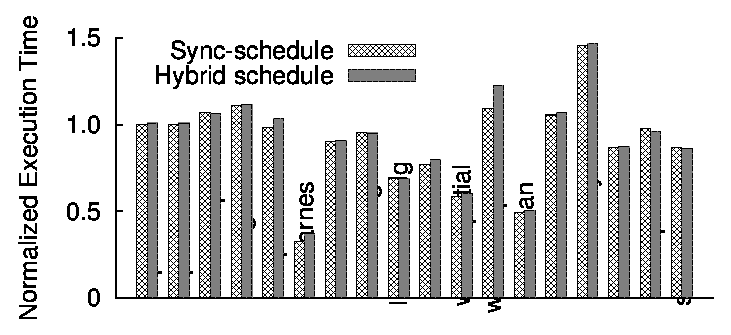
\includegraphics[width=\columnwidth]{peregrine/figures/overhead.eps}
\vspace{-.3in}
\caption{{\em Normalized execution time when reusing sync-schedules
    v.s. hybrid schedules.}  A time value greater than 1
  indicates a slowdown compared to a nondeterministic execution without
  \peregrine.  We did not include \racey because it was not designed for
  performance benchmarking. } \label{fig:peregrine-overhead}
\end{figure}

For comparison, Figure~\ref{fig:peregrine-overhead} shows the normalized
execution time when enforcing just the sync-schedules.  This overhead is
comparable to our previous work~\cite{cui:tern:osdi10}.  For all
programs except \watern, the overhead of enforcing hybrid schedules is only slightly
larger (at most 5.4\%) than that of enforcing sync-schedules.
This slight increase comes from two sources: (1) \peregrine has to enforce
execution order constraints to resolve races deterministically for \pbzip,
 \barnes, \fft, and \lun; and (2) the instrumentation framework \peregrine uses
also incurs overhead (\S\ref{sec:peregrine-enforce-schedule}). 
The overhead for \watern increases by 13.4\% because it calls functions
more frequently than the other benchmarks, and our instrumentation framework
inserts code at each function entry and return
(\S\ref{sec:peregrine-enforce-schedule}).


\begin{figure}[b!]
\centering
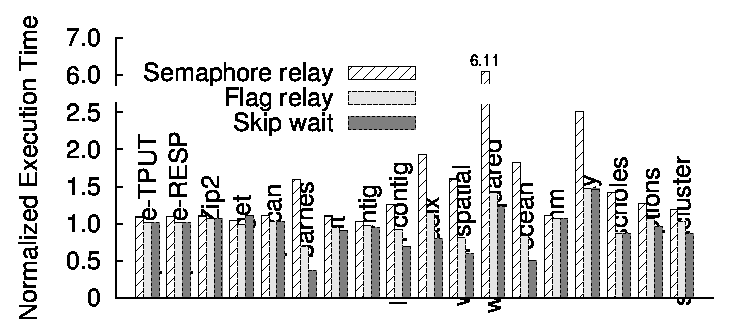
\includegraphics[width=\columnwidth]{peregrine/figures/opt.eps}
\vspace{-.3in}
\caption{{\em Speedup of optimization techniques.} Note that Y axis is
  broken.} \label{fig:peregrine-opt}
\end{figure}

Figure~\ref{fig:peregrine-opt} shows the speedup of flag relay
(\S\ref{sec:peregrine-enforce-schedule}) and skipping blocking operations
(\S\ref{sec:peregrine-nowait}).  Besides \watern and \cholesky, a
second group of programs, including \barnes, \lun, \radix, \waters, and
\ocean, also perform many synchronization operations, so flag relay speeds up
both groups of programs significantly.  Moreover, among the
synchronization operations done by the second group of programs, many are
\vv{pthread\_barrier\_wait()} operations, so \peregrine further speeds up these
programs by skipping these wait operations.



\begin{table}[!ht]
\scriptsize
\centering
\begin{tabular}{crrrrrrr}
{\bf Program} &{\bf Trace}&{\bf Det} & {\bf Sli}  & {\bf Sim} & {\bf Sym} \\
\hline                                                                   
\apache       & 449       & 0.4      & 885.32     & n/a       & 5.8       \\
\pbzip        & 2,227     & 0.1      & 587.9      & 317.8     & 19.7      \\
\aget         & 233       & 0.4      & 78.8       & 60.1      & 13.2      \\
\pfscan       & 46,602    & 1.1      & 1,601.4    & 2,047.9   & 1,136.6   \\
\barnes       & 324       & 0.2      & 300.5      & 481.5     & 56.9      \\
\fft          & 39        & 0.0      & 2.1        & 3,661.7   & 0.4       \\
\luc          & 44,799    & 19.9     & 1,271.5    & 124.9     & 1,126.7   \\
\lun          & 41,302    & 21.2     & 1,999.8    & 14,243.8  & 1,201.0   \\
\radix        & 3,110     & 1.5      & 46.2       & 96.4      & 182.9     \\
\waters       & 7,508     & 1.0      & 1,407.0    & 9,628.1   & 120.6     \\
\watern       & 12,381    & 1.7      & 962.3      & 1,841.4   & 215.7     \\
\ocean        & 55,247    & 26.4     & 2,259.3    & 5,902.8   & 2,062.1   \\
\fmm          & 13,772    & 8.3      & 260.5      & 1,107.5   & 151.3     \\
\cholesky     & 47,200    & 28.8     & 3,102.9    & 6,350.1   & 685.5     \\
\blackscholes & 62,024    & 16.5     & 539.9      & 542.9     & 3,284.8   \\
\swaptions    & 1,366     & 0.0      & 23.2       & 87.3      & 1.2       \\
\streamcluster& 259       & 0.1      & 1.4        & 1.9       & 4.9       \\ 
\end{tabular}
\caption{{\em Analysis time.} {\bf Trace} shows the number of thousand
  LLVM instructions in the execution trace of the evaluated programs,
  the main factor affecting the execution time of \peregrine's various analysis
  techniques, including race detection ({\bf Det}), slicing ({\bf Sli}),
  simplification and alias analysis ({\bf Sim}), and symbolic execution
  ({\bf Sym}).  The execution time is measured in seconds.  The \apache
  trace is collected from one window of eight requests.  \apache uses
  thread pooling which our simplification technique currently does not
  handle well (\S\ref{sec:peregrine-window}); nonetheless, slicing without simplification
  works reasonably well for \apache already
  (\S\ref{sec:peregrine-stable}).} \label{tab:peregrine-analysis-overhead}
\end{table}


\para{Analyzer and recorder overhead.}  Table~\ref{tab:peregrine-analysis-overhead}
shows the execution time of \peregrine's various program analyses.  The
execution time largely depends on the size of the execution trace.  All
analyses typically finish within a few hours.  For \pbzip and \fft, we
used small workloads (compressing 1~KB file and transforming a 256X256
matrix) to reduce analysis time and to illustrate that the schedules
learned from small workloads can be efficiently reused on large workloads.
The simplification and alias analysis time of \fft is large compared to its
slicing time because it performs many multiplications on array indexes,
slowing down our range analysis.  Although \lun and \luc implement the
same scientific algorithm, their data access patterns are very different
(\S\ref{sec:peregrine-stable}), causing \peregrine to spend more time analyzing \lun than \luc.

\begin{figure}[b!]
\centering
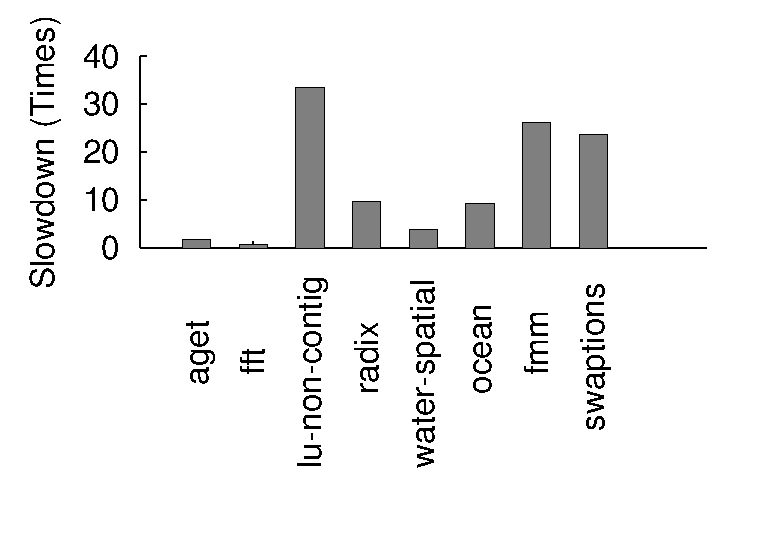
\includegraphics[width=.7\columnwidth]{peregrine/figures/new-recorder.eps}
\vspace{-.25in}
\caption{{\em Overhead of recording \vv{load} and \v{store} instructions.}} \label{fig:peregrine-new-recorder-overhead}
\end{figure}

As discussed in \S\ref{sec:peregrine-record}, \peregrine currently runs \klee to record
executions.  Column Sym is also the overhead of \peregrine's recorder.  This
crude, unoptimized recorder can incur large slowdown compared to
the normal execution of a program.  However, this slowdown can be reduced
to around 10X using existing record-replay
techniques~\cite{idna:vee06,scribe:sigmetrics10}.  Indeed, we have
experimented with a preliminary version of a new recorder that records an
execution by instrumenting \vv{load} and \v{store} instructions and saving
them into per-thread logs~\cite{idna:vee06}.  Figure~\ref{fig:peregrine-new-recorder-overhead} shows that
this new recorder incurs roughly 2-35X slowdown on eight programs,
comparable to existing record-replay systems.  Due to time
constraints, we have not integrated this new recorder with \peregrine.



\subsection{Stability} \label{sec:peregrine-stable}

Stability measures how frequently \peregrine can reuse schedules.  The more
frequently \peregrine reuses schedules, the more efficient it is, and the
more repeatable a program running on top of \peregrine becomes.  While \peregrine
achieves determinism and efficiency through hybrid schedules, it may have
to pay the cost of slightly reduced reuse rates compared to a
manual approach~\cite{cui:tern:osdi10}.




\begin{figure}[t]
\centering
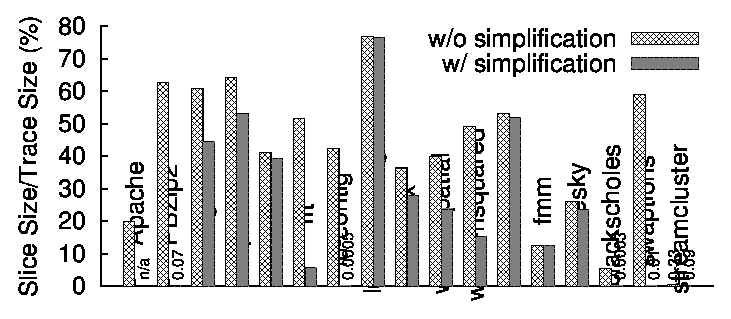
\includegraphics[width=\columnwidth]{peregrine/figures/slicing.eps}
\vspace{-.3in}
\caption{{\em Slicing ratio after applying determinism-preserving slicing alone 
    (\S\ref{sec:slice}) and after further applying schedule-guided
    simplification (\S\ref{sec:peregrine-guide}).}} \label{fig:peregrine-slice-ratio}
\vspace{-.05in}
\end{figure}

A key factor determining \peregrine's schedule-reuse rates is how effectively it
can slice out irrelevant instructions from the execution traces.
Figure~\ref{fig:peregrine-slice-ratio} shows the ratio of the slice size over the trace size for
\peregrine's determinism-preserving slicing technique, with and without
schedule-guided simplification.  The slicing technique alone reduces the
trace size by over 50\% for all programs except \pbzip, \aget, \pfscan,
\fft, \lun, \ocean, and \swaptions.  The slicing technique combined with
scheduled-guide simplification vastly reduces the trace size for \pbzip,
\aget, \fft, \luc, and \swaptions.

Recall that \peregrine computes the preconditions of a schedule from
the input-dependent branches in a trace slice.  The
fewer branches included in the slice, the more general the preconditions
\peregrine computes tend to be.  We further measured the number of such
branches in the trace slices.  Table~\ref{tab:peregrine-slice-ratio} shows the
results, together with a upper bound determined by the total number of
input-dependent branches in the execution trace, and a lower bound
determined by only including branches required to reach the recorded
synchronization operations.  This lower bound may not be tight as we ignored data
dependency.  For \barnes, \fft, \blackscholes, \swaptions, and
\streamcluster, slicing with simplification (Column ``Slicing+Sim'')
achieves the best possible reduction.  For \pbzip, \aget, \pfscan, and \luc, the
number of input-dependent branches in the trace slice is close to the
lower bound.  In the remaining programs, \apache, \fmm, and \cholesky
also enjoy large reduction, while the other five programs do not.  This table
also shows that schedule-guided simplification is key to reduce the
number of input-dependent branches for \pbzip, \fft, \luc, \blackscholes, 
and \swaptions,
and to reach the lower bound for \blackscholes, \swaptions, and \streamcluster.


We manually examined the preconditions \peregrine computed from the
input-dependent branches for these programs.  We category these programs
below.

\para{Best case}: \pbzip, \fft, \luc, \blackscholes, \swaptions,
  and \streamcluster. \peregrine computes the weakest (\ie, most relaxed) preconditions
  for these programs.  The preconditions often allow \peregrine to reuse
  one or two schedules for each number of threads, putting no
   or few constraints on the data processed.
  Schedule-guided simplification is crucial for
  these programs; without simplification, the preconditions
  would fix the data size and contents.

\para{Slicing limitation}: \apache and \aget. The
  preconditions \peregrine computes for \apache fix the URL length; they also
  constrain the page size to be within an 8~KB-aligned range if
    the page is not cached.  The preconditions \peregrine computes for \aget fix
    the positions of ``\vv{/}'' in the URL and narrow down the file size
    to be within an 8~KB-aligned range.  These preconditions thus
      unnecessarily reduce the schedule-reuse rates.  Nonetheless, they
      can still match many different inputs, because they do not constrain
      the page or file contents.

\para{Symbolic execution limitation}: \barnes.  \barnes
  reads in two floating point numbers from a file, and their values affect
  schedules.  Since \peregrine cannot symbolically execute floating point
  instructions, it currently does not collect preconditions from them.

\para{Alias limitation}: \lun, \radix, \waters, \watern, \ocean,
  and \cholesky.  Even with simplification, \peregrine's alias analysis
  sometimes reports may-alias for pointers accessed in different threads,
  causing \peregrine to include more instructions than necessary in the
  slices and compute preconditions that fix the input data.  For
  instance, each thread in \lun accesses disjoint regions in a global
  array, but the accesses from one thread are \emph{not} continuous,
  confusing \peregrine's alias analysis.  (In contrast, each thread in \luc accesses
  a contiguous array partition.)

\para{Programs that rarely reuse schedules}: \pfscan and
  \fmm.  For instance, \pfscan searches a keyword in a set of files using
  multiple threads, and for each match, it grabs a lock to increment a
  counter.  A schedule computed on one set of files is unlikely to suit
  another.

\begin{table}[!ht]
\small
\centering
\begin{tabular}{crrrr}
\multirow{2}{*}{\bf Program} & \multirow{2}{*}{\bf UB} 
& \multicolumn{2}{c}{\bf \peregrine} 
& \multirow{2}{*}{\bf LB} \\
& & {\bf Slicing} & {\bf Slicing+Sim} & \\
\hline
\apache       &  4,522   &  624    & n/a      & 56     \\
\pbzip        &  913     &  865    & 101      & 94     \\
\aget         & 20,826   & 18,859  & 9,514    & 9,491  \\
\pfscan       & 1,062,047& 992,524 & 992,520  & 992,501\\
\barnes       &  92      & 52      & 52       & 52     \\
% This is fft -p8 -m6 slicing results, not m16. Range analysis currently can not run m16.
\fft          &  2,266   & 1,568   & 17       & 17     \\
\luc          &2,823,379 &2,337,431& 131      & 128    \\
\lun          &2,962,621 &2,877,877& 2,876,364& 128    \\
\radix        &  175,679 & 98,750  & 89,732   & 75     \\
\waters       &  98,054  & 77,567  & 76,763   & 233    \\
\watern       &  89,348  & 76,786  & 76,242   & 1,843  \\
\ocean        &2,605,185 &2,364,538&2,361,256 & 400    \\
\fmm          &  299,816 & 57,670  & 56,532   & 1,642  \\
\cholesky     &  7,459   & 1,627   & 1,627    & 1,233   \\
\blackscholes & 421,909  & 409,618 & 10       & 10 \\
\swaptions    & 35,584   & 35,005  & 21       & 21 \\
\streamcluster& 20,851   & 75      & 42       & 42 \\
\end{tabular}
\vspace{-.1in}
\caption{{\em Effectiveness of program analysis techniques.}  {\bf UB}
  shows the total number of input-dependent branches in the
  corresponding execution trace, an upper bound on the number included in 
  the trace slice.  {\bf Slicing} and {\bf Slicing+Sim} show the
  number of input-dependent branches in the slice after applying
  determinism-preserving slicing alone (\S\ref{sec:peregrine-slice}) and after
  further applying schedule-guided simplification
  (\S\ref{sec:peregrine-guide}). {\bf LB} shows a lower bound on the number of
  input-dependent branches, determined by only including branches
  required to reach the recorded synchronization operations.
  This lower bound may not be tight as we ignored data
  dependency when computing it.} \label{tab:peregrine-slice-ratio}
\vspace{-.05in}
\end{table}




\subsection{Ease of Use} \label{sec:peregrine-annotation}

\begin{table}[!ht]
\centering
\small
\begin{tabular}{crcc}
{\bf Program} & {\bf LOC} & {\bf \peregrine} & {\bf \tern} \\
\hline
% -6.0 
\apache       & 464~K   & 24  & 6  \\
\pbzip        & 7,371  & 1   & 3  \\
\aget         &   834  & 0   & n/a\\
\pfscan       &   776  & 0   & n/a\\
\barnes       & 1,954  & 0   & 9  \\
\fft          & 1,403  & 1   & 4  \\   
\luc          & 991    & 0   & n/a  \\ 
\lun          & 1,265  & 0   & 3  \\   
\radix        & 661    & 0   & 4  \\   
\waters       & 1,573  & 0   & 9  \\
\watern       & 1,188  & 0   & 10 \\
\ocean        & 6,494  & 0   & 5  \\
\fmm          & 3,208  & 0   & 9  \\
\cholesky     & 3,683  & 0   & 4  \\
\blackscholes & 1,275  & 0   & n/a\\
\swaptions    & 1,110  & 0   & n/a\\
\streamcluster& 1,963  & 0   & n/a\\
\racey        & 124    & 0   & n/a\\
\end{tabular}
\vspace{-.05in}
\caption{{\em Source annotation requirements of \peregrine v.s. \tern.}  {\bf
    \peregrine} represents the number of annotations added for \peregrine, and {\bf
    \tern} counts annotations added for \tern.  Programs not included in
  the \tern evaluation are labeled n/a. LOC of \pbzip also includes the
  lines of code of the compression library \vv{libbz2}.} \label{table:peregrine-apps}
\vspace{-.05in}
\end{table}

Table~\ref{table:peregrine-apps} shows the annotations (\S\ref{sec:peregrine-func-summary}) we
added to make the evaluated programs work with \peregrine.  For most programs,
\peregrine works out of the box.  \apache uses its own library functions for
common tasks such as memory allocation, so we annotated 21 such
functions.  We added two annotations to mark the boundaries of client
request processing and one to expose the hidden state
in \apache (\S\ref{sec:peregrine-window}).  \pbzip decompression
uses a custom search function (\vv{memstr}) to scan through the input file
for block boundaries.  We added one annotation for this function to relax
the preconditions \peregrine computes.  (\peregrine works automatically with \pbzip
compression.)  We added one assertion to annotate the range of a variable
in \fft (\S\ref{sec:peregrine-func-summary}).

For comparison, Table~\ref{table:peregrine-apps} also shows the annotation overhead of our previous DMT system \tern~\cite{cui:tern:osdi10}.  For all programs except \apache, \peregrine
has fewer number of annotations than \tern.  Although the number
of annotations that \tern has is also small, adding these annotations may
require developers to manually reconstruct the control- and
data-dependencies between instructions.


% emphasize interesting side effects
In order to make the evaluated programs work with \peregrine, we had to fix several bugs
in them.  For \aget, we fixed an off-by-one write in \vv{revstr()} which
prevented us from tracking constraints for the problematic write, and a
missing check on the return value of \vv{pwrite()} which prevented us from
computing precise ranges.  We fixed similar missing checks in \swaptions,
\streamcluster, and \radix.  We did not count these modifications in
Table~\ref{table:peregrine-apps} because they are real bug fixes.  (This interesting
side-effect illustrates the potential of \peregrine as an error detection tool:
the precision gained from simplification enables \peregrine to detect real races
in well-studied programs.)



\section{Related Work} \label{sec:peregrine-related}

\para{\smt and \dmt systems.}
\peregrine stabilizes program behaviors over input perturbations by reusing 
schedules. This method is based on the \emph{schedule-memoization} idea in our 
previous system \tern~(Chapter~\ref{sec:tern}), but \peregrine largely 
eliminates manual annotations, and provides stronger determinism guarantees than 
\tern.

\peregrine is complementary to other \smt and \dmt 
systems~\cite{determinator:osdi10, dthreads:sosp11, cui:tern:osdi10, 
coredet:asplos10, kendo:asplos09, dmp:asplos09}: \peregrine can use an
existing \smt or \dmt algorithm when it runs a program on a new input
so that it may compute the same schedules at different sites;
existing \smt or \dmt systems can speed up their pathological cases
using the schedule-relaxation idea.

Determinator~\cite{determinator:osdi10}
advocates a new, radical programming model that converts all races,
including races on memory and other shared resources, into exceptions, to
achieve pervasive determinism. This programming model is not designed to
be backward-compatible. dOS~\cite{dos:osdi10} provides similar pervasive
determinism with backward compatibility, using a \dmt algorithm first
proposed in~\cite{dmp:asplos09} to enforce mem-schedules.  While \peregrine
currently focuses on multithreaded programs, the ideas in \peregrine can be
applied to other shared resources to provide pervasive determinism.
\peregrine's hybrid schedule idea may help reduce dOS's overhead.  
Grace~\cite{grace:oopsla09} makes multithreaded programs with fork-join 
parallelism behave like sequential programs.  It detects memory access 
conflicts efficiently using hardware page protection.  Unlike Grace, \peregrine 
aims to make general multithreaded programs, not just fork-join programs, 
repeatable.

Concurrent to our work, \dthreads~\cite{dthreads:sosp11} is another
efficient multithreading system that is both stable and deterministic. It 
tracks memory modifications using hardware page protection and provides a 
protocol to deterministically commit these modifications. In contrast to 
\dthreads, \peregrine is software-only and does not rely on page protection 
hardware which may be expensive and suffer from false sharing; \peregrine 
records and reuses schedules, thus it can handle programs with ad hoc 
synchronizations~\cite{syncfinder:osdi10} and make program behaviors stable.

\para{Program analysis.}  Program slicing~\cite{Tip:slicing} is a general
technique to prune irrelevant statements from a program or trace.
Recently, systems researchers have leveraged or invented slicing
techniques to block malicious input~\cite{castro:bouncer}, synthesize
executions for better error diagnosis~\cite{esd:eurosys10}, infer source
code paths from log messages for postmortem
analysis~\cite{sherlog:asplos10}, and identify critical inter-thread reads
that may lead to concurrency errors~\cite{conseq:asplos11}.  
Our determinism-preserving slicing technique produces a correct trace slice for
multithreaded programs and supports multiple ordered targets.  It thus has
the potential to benefit existing systems that use slicing.  

Our schedule-guided simplification technique shares similarity with
SherLog~\cite{sherlog:asplos10} such as the removal of branches
contradicting a schedule.  However, SherLog starts from log messages and
tries to compute an execution trace, whereas \peregrine starts with a schedule
and an execution trace and computes a simplified yet runnable program.
\peregrine can thus transparently improve the precision of many existing
analyses: simply run them on the simplified program.


\para{Replay and re-execution.}  Deterministic
replay~\cite{r2:osdi, friday2007, srinivasan:flashback, revirt, dejavu, 
vmware-record-replay, smp-revirt:vee08, pres:sosp09, scribe:sigmetrics10, 
odr:sosp09, capo:asplos09} aims to replay the exact recorded executions, 
whereas \peregrine ``replays" schedules on different inputs.  Some recent 
deterministic replay systems include Scribe, which tracks page ownership to 
enforce deterministic memory access~\cite{scribe:sigmetrics10}; Capo, which 
defines a novel software-hardware interface and a set of abstractions for 
efficient
replay~\cite{capo:asplos09}; PRES and ODR, which systematically search for
a complete execution based on a partial one~\cite{pres:sosp09, odr:sosp09};
SMP-ReVirt, which uses page protection for recording the
order of conflicting memory accesses~\cite{smp-revirt:vee08}; and
Respec~\cite{respec:asplos10}, which uses online replay to keep multiple
replicas of a multithreaded program in sync.  Several
systems~\cite{pres:sosp09,respec:asplos10} share the same insight as \peregrine:
although many programs have races, these races tend to occur infrequently.

\peregrine can help these systems reduce CPU, disk, or network bandwidth
overhead, because for inputs that hit \peregrine's schedule cache, these systems
do not have to record a schedule.

Retro~\cite{retro:osdi10} shares some similarity with \peregrine because it also
supports ``mutated'' replay.  When repairing a compromised system, Retro
can replay legal actions while removing malicious ones using a novel
dependency graph and \emph{predicates} to detect when changes to an object
need not be propagated further.  \peregrine's determinism-preserving slicing
algorithm may be used to automatically compute these predicates, so that
Retro does not have to rely on programmer annotations. 


\para{Concurrency errors.} The complexity in developing multithreaded
programs has led to many concurrency errors~\cite{lu:concurrency-bugs}.
Much work exists on concurrency error
detection, diagnosis, and correction 
(\eg,~\cite{yu:racetrack:sosp,racerx:sosp03,lu:muvi:sosp,conmem:asplos10,
conseq:asplos11,2ndstrike:asplos11,linearizable:eurosys11,ctrigger:asplos09}).  
\peregrine aims to make the
executions of multithreaded programs repeatable, and is complementary to
existing work on concurrency errors.  \peregrine may use existing
work to detect and fix the errors in the schedules it computes.
Even for programs free of concurrency errors, \peregrine still provides value by
making their behaviors repeatable.




\section{Summary} \label{sec:peregrine-summary}

\peregrine is one of the first efficient and fully deterministic multithreading systems.
Leveraging the insight that races are rare, \peregrine combines sync-schedules
and mem-schedules into hybrid schedules, getting the benefits of both.
\peregrine reuses schedules across different inputs, amortizing the cost of
computing hybrid schedules and making program behaviors repeatable
across inputs.  It further improves
efficiency using two new techniques: determinism-preserving slicing to
generalize a schedule to more inputs while preserving determinism, and
schedule-guided simplification to precisely analyze a program according
to a dynamic schedule.  Our evaluation on a diverse set of programs
shows that \peregrine is both deterministic and efficient, and can frequently
reuse schedules for half of the evaluated programs.

%% We have presented \peregrine, an efficient deterministic multithreading system
%% designed for general multithreaded programs and commodity hardware.  The
%% key insight in \peregrine is that although programs have races, these races tend
%% to occur only for minor portions of an execution, and the majority of the
%% execution is still race-free.  Based on this insight, \peregrine enforces a
%% mem-schedule only for the racy portions of an execution and a
%% sync-schedule otherwise, thus combining the efficiency of sync-schedules
%% and determinism of mem-schedules.  \peregrine computes a hybrid schedule by
%% relaxing a fine-grained execution trace, and reuses this schedule on
%% future inputs when possible.  


\peregrine's system and ideas have broad applications.  Our immediate future
work is to build applications on top of \peregrine, such as fast deterministic replay,
replication, and diversification systems.  We will also extend our
approach to system-wide deterministic execution by computing inter-process
communication schedules and preconditions.  \peregrine enables precise program
analysis according to a set of inputs and dynamic schedules.  We will
leverage this capability to accurately detect concurrency errors and
verify concurrency-error-freedom for real programs.




\section{\parrot: Making \smt Simple and Deployable} \label{sec:parrot}

Although the latest advances on building stable
multi-threading systems are promising, whether \smt systems can be 
made simple and deployable stills remains an open challenges. Existing systems 
either incur high performance overhead~cite{dthreads:sosp11} (For instance, 
we observed that a prior system, \dthreads, had 5$\times$ to 100$\times$ slowdown on
some programs), or require sophiscated program analysis~cite{peregreine:sosp11, bergan:oopsla13}
and fairly hard to deploy.
These limitations make evaluation in existing systems limited: they often 
used (1) synthetic benchmarks,
not real-world programs, from incomplete benchmark suites; (2) one workload
per program; and (3) at most 8 cores (with three exceptions; see \S\ref{sec:
related}).

These limitations are intermingled.  Reducing schedules improves correctness
but trades performance because the schedules left may not balance each
thread's load well, causing some threads to idle unnecessarily.  Our
experiments show that ignoring load imbalance as in \dthreads
can lead to pathological
slowdown if the order of operations enforced by a schedule
\emph{serializes} the intended parallel computations.
To recover performance, one method is to count
the instructions executed by each thread and select schedules that balance
the instruction counts~\cite{kendo:asplos09, coredet:asplos10,
  dmp:asplos09}, but this method is not stable because input or program
perturbations easily change the instruction counts.  The other method (we 
proposed)
lets the nondeterministic OS scheduler select
a reasonably fast schedule and reuses the schedule on
compatible inputs~\cite{cui:tern:osdi10,peregrine:sosp11}, but it
requires sophisticated program analysis, complicating deployment.

We present \parrot, a simple, deployable runtime that efficiently makes
threads deterministic and stable by offering a new contract to developers.
By default, it schedules synchronizations in each thread using
round-robin, vastly reducing schedules and providing broad repeatability.
When default schedules are slow, it allows advanced developers to add
intuitive \emph{performance hints} to their code for speed.  Developers 
discover
where to add hints through profiling as usual, and \parrot simplifies
performance debugging by deterministically reproducing the bottlenecks.
The hints are robust to developer mistakes as they can be safely ignored
without affecting correctness.

Like prior systems, \parrot's contract reduces schedules to favor correctness 
over performance.  Unlike prior systems, it allows advanced developers
to optimize performance.  We believe this practical ``meet in the
middle'' contract eases writing correct, efficient programs.

% based on several years of lessons.

%% Like prior systems, \parrot's contract favors correctness over performance
%% by vastly reducing schedules.  Unlike prior systems, it provides
%% advanced developers the flexibility for better performance.

\parrot provides two performance hint abstractions.  A \emph{soft
  barrier} encourages the scheduler to coschedule a group of threads at
given program points.  It is for performance only, and operates as a
barrier with deterministic timeouts in \parrot.  Developers use it to switch
to faster schedules without compromising determinism
when the default schedules serialize parallel
computations.  A \emph{performance critical section}
informs the scheduler that a code region is a potential
bottleneck, encouraging the scheduler to get through the region fast.
When a thread enters a performance critical section, \parrot delegates 
scheduling to the
nondeterministic OS scheduler for speed.  
Performance critical sections may trade some determinism for
performance, so they should be applied only when the schedules they add
are thoroughly checked by tools or advanced developers.
These simple abstractions
let \parrot run fast on all programs evaluated, and
may benefit other DMT or \smt systems and classic nondeterministic
schedulers~\cite{coschedule:sigmetrics96, coschedule, partial-barrier:atc06}.

Our \parrot implementation is \pthread-compatible, simplifying deployment.
It handles many diverse constructs real-world programs depend upon such as
network operations and timeouts.  \parrot makes synchronizations outside
performance critical sections deterministic but allows nondeterministic
data races.  Although it is
straightforward to make data races deterministic in \parrot,
% with a memory commit protocol we designed, 
we deemed it not worthwhile because the cost of doing so outweighs the
benefits.  \parrot's determinism is similar to
\kendo's weak determinism~\cite{kendo:asplos09}, but \parrot offers stability
which Kendo lacks.

\subsection{Evaluation} \label{sec:parrot-eval}

In this evaluation, we focus on examing \parrot's practicality by running it 
with a wide range of popular-multithreaded programs, check whether \parrot is 
easy to use with these programs, and collect \parrot's 
execution time on utlity programs and throughput on server programs.

We evaluated \parrot on a diverse set of \nprog programs. This set
includes \nrealprog real-world programs: \bdb, a widely used database
library~\cite{berkeleydb}; \openldap, a server implementing the
Lightweight Directory Access Protocol~\cite{openldap}; \redis, a fast
key-value data store server~\cite{redis}; \mplayer, a popular media
encoder, decoder, and player~\cite{mplayer}; \pbzip, a parallel
compression utility~\cite{pbzip2}; \pfscan, a parallel \v{grep}-like
utility~\cite{pfscan}; \aget, a parallel file download
utility~\cite{aget}; all \nstl parallel C++ STL algorithm
implementations~\cite{parallel-stl} which use \openmp; all \nimagick
parallel image processing utilities (which also use \openmp) in the
\imagick software suite~\cite{imagick} to create, edit, compose, or
convert bitmap images.  The set also includes all \nbenchmarks programs in
four widely used benchmark suites including \nparsec in
\parsec~\cite{parsec}, \nphoenix in
\phoenix~\cite{phoenix-benchmarks}, \nsplash in
\splashx~\cite{splashx}, and \nnpb in \npb~\cite{npb}.  The \phoenix
benchmark suite provides two implementations per algorithm, one using
regular Pthreads (marked with \v{-pthread} suffix) and the other using
a map-reduce library atop Pthreads.  We used complete software or
benchmark suites to avoid biasing our results.  The programs together
cover a good range of parallel programming models and idioms such as
threads, \openmp, data partition, fork-join, pipeline, map-reduce, and
workpile.  To the best of our knowledge, our evaluation of \parrot
represents \overeach more programs than any prior DMT or \smt
evaluation, and \overcombined more than all prior
evaluations combined.

Our evaluation machine was a 2.80 GHz dual-socket hex-core Intel Xeon
with 24 hyper-threading cores and 64 GB memory
running Linux 3.2.14.  Unless otherwise specified, we used the maximum
number of truly concurrent threads allowed by the machine and programs.  For 83
out of the \nprog programs, we used 24.  For 13 programs, we used 16
because they require the number of threads be a power of 
two. For \ferret, we used 18 because it requires
the number of threads to be 4$n$+2. For \mplayer, we used 8,
the max it takes. For the other
10 programs, we used 16 because they reach peak performance with
this thread count.  In scalability experiments, we varied the number of
threads from 4 to the max.



Unless otherwise specified, we used the following workloads.  For \bdb, we
used a popular benchmark \v{bench3n}~\cite{benchthreen}, which does
fine-grained, highly concurrent transactions. For both \openldap and
\redis, we used the benchmarks the developers themselves use, which come
with the code. For \mplayer, we used its utility \mencoder to transcode a
255 MB video (OSDI '12 keynote) from MP4 to AVI.  For \pbzip, we
compressed and decompressed a 145 MB binary file.  For \pfscan, we searched for
the keyword \v{return} in all 16K files in \v{/usr/include} on our
evaluation machine.  For \aget, we downloaded a 656 MB file. For all
\imagick programs, we used a 33 MB JPG.  For all \nstl
parallel STL algorithms, we used integer vectors with 4G elements.  For
\parsec, \splashx, and \phoenix, we used the largest workloads
because they are considered ``real'' by the benchmark authors.  For \npb, we
used the second largest workloads because the largest workloads are intended 
for
supercomputers. In workload sensitivity experiments, we used workloads of
3 or 4 different scales per program, typically with a 10$\times$ difference 
between
scales.  We also tried 15 different
types of workloads for \redis and 5 for \mplayer.  All workloads ran from
a few seconds to about 0.5 hour, using 100 or 10
repetitions respectively to bring the standard error below 1\%.
All overhead means are geometric.

We compiled all programs using \v{gcc -O2}.  To support
\openmp programs such as parallel STL algorithms, we used the GNU \libgomp.
When evaluating \parrot on the client program \aget and the server programs \
openldap
and \redis, we ran both endpoints on the same machine to avoid network
latency.  \nprogadhocsync programs use ad hoc
synchronization~\cite{syncfinder:osdi10}, and we added a \v{sched\_yield}
to the busy-wait loops to make the programs work with \parrot. We set the
spin-wait of \parrot's scheduler
to $10^5$ cycles.  We used the default \compute timeout of 20 except 3,000
for \ferret.  Some \phoenix programs read large files, so
we ran them with a warm file cache to focus on measuring their computation
time. (Cold-cache results are unusable due to large
variations~\cite{Parrot:github}.)



\subsection{Ease of Use} \label{sec:parrot-use}

Of all \nprog programs, \nprognohints have reasonable overhead with
default schedules, requiring no hints.  \nproglineuphints programs need a 
total of 
\nlineofcomputehints lines of \compute hints: \nproggenericlineuphints
need only 4 lines of generic \compute hints in \libgomp, and
\nprogspecificlineuphints need program-specific \computes
(Table~\ref{tab:computehints}).  These programs enjoy both determinism and
reasonable performance.  Only \nprognondethints programs 
need a total of \nlineofnondethints lines of \nondet hints to
trade some determinism for performance (Table~\ref{tab:nondethints}).
On average, each program needs only \hintsperprog lines.


In our experience, adding hints was straightforward.  It took roughly 0.5--2 
hours per program despite unfamiliarity with the programs.  We believe
the programs' developers would spend much less time adding better hints.
\parrot helped us deterministically reproduce the bottlenecks and identify
the synchronizations delayed by round-robin.  We used Intel \vtune~\cite{vtune} and
Linux \v{perf}~\cite{perf} performance counter-based tools to identify time-
consuming computations, and usually needed to align only the top two or three
computations.  For instance, \ferret uses a pipeline of six stages, all
serialized by the \parrot's default schedules.  We aligned only two of them to 
bring the overhead down to a reasonable level.  Aligning more stages did not help.










\begin{table}[t]
\footnotesize
\centering
\begin{tabular}{lr}
{\bf Program} & {\bf Lines} \\
\hline

\mencoder, \vips, \swaptions, \freqmine, \facesim
,                                 &   2 each  \\
\xtwosixfour, \radiosity, \radix, \kmeans, \\
\linearregrepthread, \linearregre, \\
\matrixmultpthread, \matrixmult, \\
\wordcntpthread, \stringmatchpthread, \\
\stringmatch, \histogrampthread, \histogram \\

\hline

\pbzip, \ferret,                                  &   3 each   \\
\kmeanspthread, \pcapthread, \pca, \wordcnt \\

\hline

\libgomp, \bodytrack  &   4 each  \\

\hline

\imagick (12 programs)                          &   25 total  \\

\end{tabular}
\caption{{\em Stats of \compute hints.} \nproglineuphints
  programs need \compute hints.  The hints in \libgomp benefit all \openmp
  programs including \imagick, STL, and \npb.} \label{tab:computehints}
\end{table}

\begin{table}[t]
\footnotesize
\centering
\begin{tabular}{lrl}
{\bf Program} & {\bf Lines} & {\bf Nondet Sync Var} \\
\hline

\pfscan                       &   2   &   \v{matches\_lock}   \\

\partition                &   2  &   \v{\_\_result\_lock}   \\

%% mutex array name: mutex[][].
\fluidanimate          &   6  &   \v{mutex[i][j]} \\

%% mutex array name: lock_array[].
\fmm                  &   2   &  \v{lock\_array[i]} \\

%% mutex array name: tasks[i].taskLock, i is thread id.
\cholesky             &   2   &  \v{tasks[i].taskLock} \\
\raytrace             &   2   &  \v{ridlock}   \\

%% mutex array name: tlock[].
\ua                       &   6   &  \v{tlock[i]} \\

\end{tabular}
\caption{{\em Stats of \nondet hints.} \nprognondethints programs need \nondet
  hints. The hints in \partition are generic for three STL programs
  \partition, \nthelement, and \partialsort. The last column shows the
  synchronization variables whose operations are made
  nondeterministic.} \label{tab:nondethints}
\end{table}

\subsection{Performance} \label{sec:parrot-performance}

\begin{figure*}[tb]
\centering
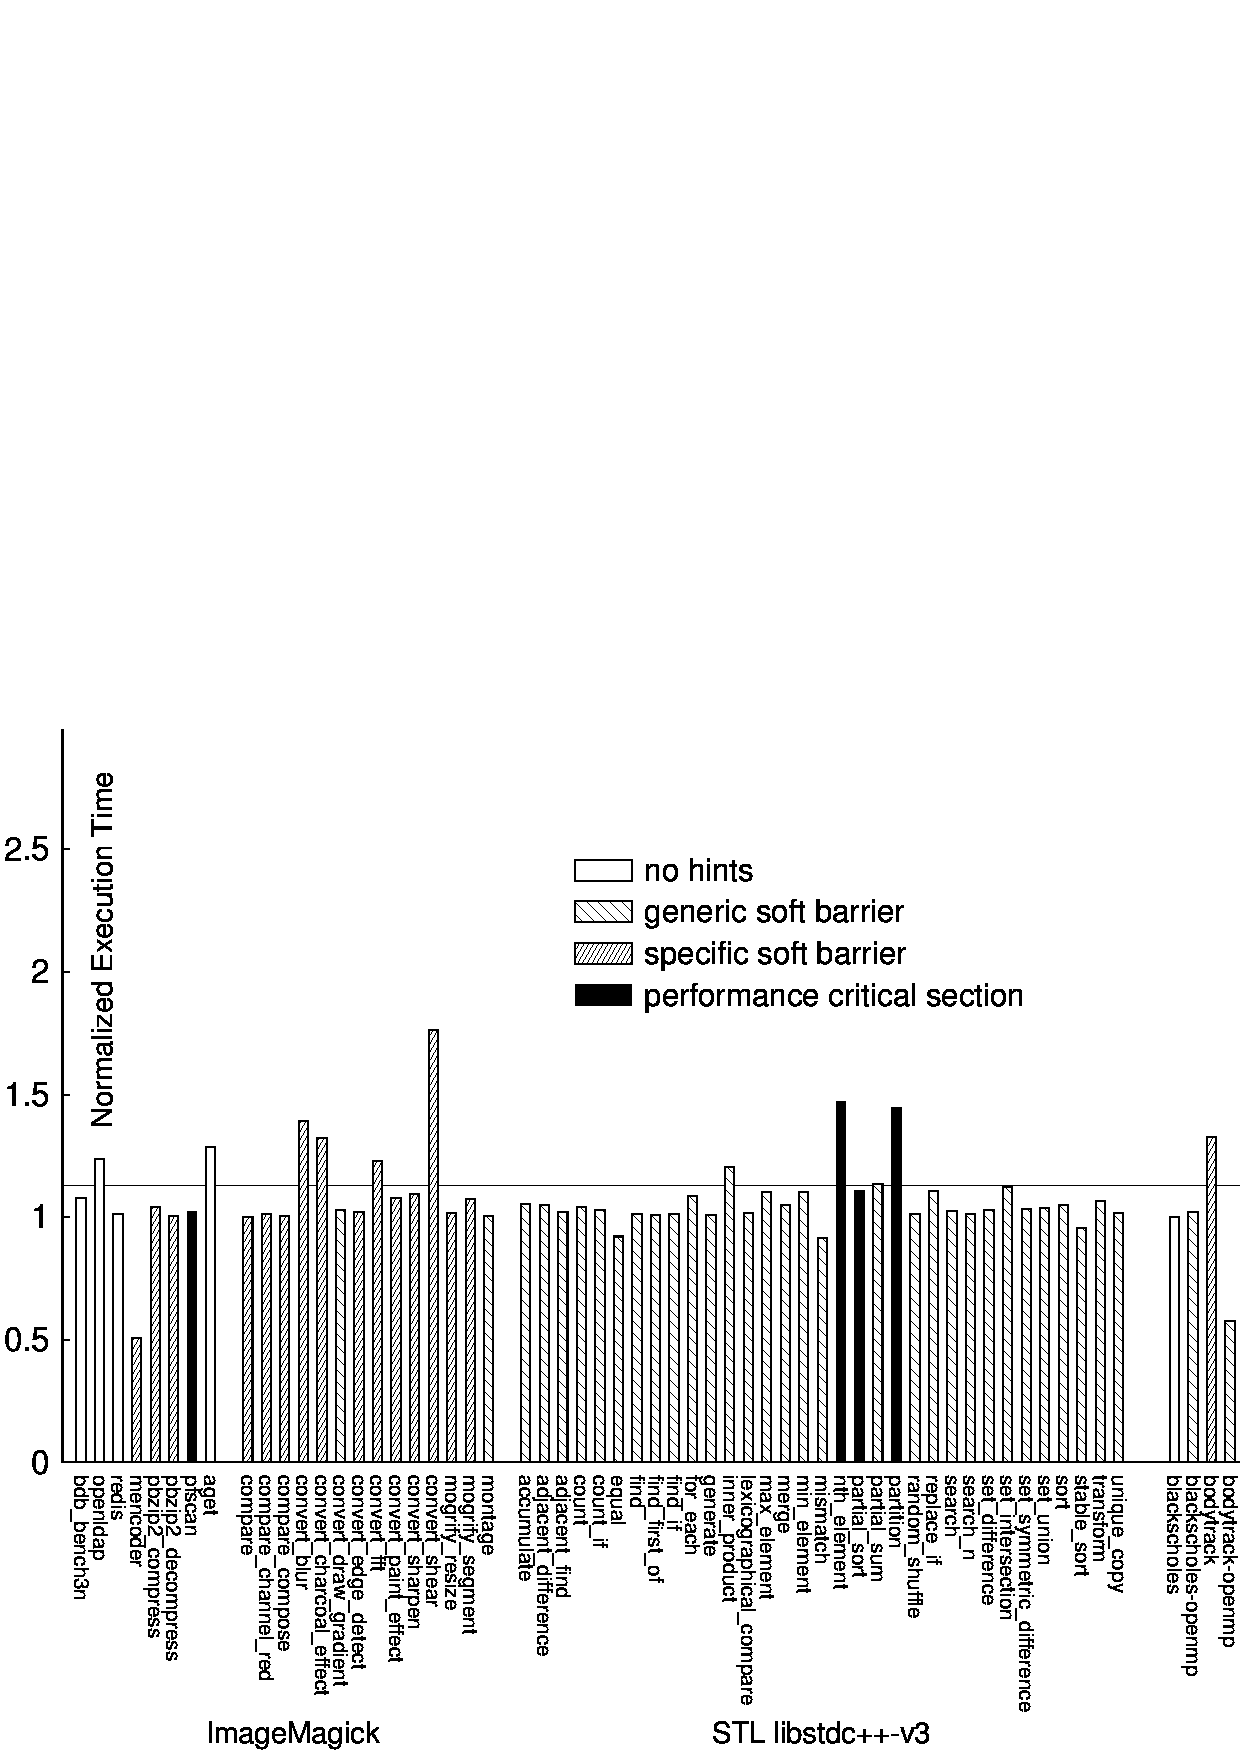
\includegraphics[width=\textwidth]{parrot/figures/overhead}
\vspace{-.20in}
\caption{{\em \parrot's performance normalized over nondeterministic
    execution.}  The patterns of the bars show the types of the hints the 
programs
  need: no hints, generic \computes in \libgomp, program-specific
  \computes, or \nondets.  The mean overhead is
  \meanoverhead (indicated by the horizontal line).} \label{fig:overhead}
\vspace{-.05in}
\end{figure*}

Figure~\ref{fig:overhead} compares \parrot's performance to nondeterministic
execution.  Even with the maximum number of threads (16--24), the mean
overhead is small: \meanrealoverhead for real-world programs, \
meanbenchoverhead for benchmark
programs, and \meanoverhead for all programs.
Only seven programs had over 100\% overhead.  The \ferret, \freqmine, and \is 
benchmarks
had dynamic load imbalance even with the starting points of the computations
aligned with \compute hints. \ua also had load 
imbalance even after \nondet hints are added.
\xtwosixfour is a pipeline program, and its overhead
comes from the \compute timeouts during the pipeline startup and
teardown.  \rtviewraytrace and \barnes have low-level
synchronizations in tight loops, and their overhead may be further reduced
with \nondets.  Four programs, \mencoder, \bodytrackopenmp, \facesim, and
\linearregrepthread, enjoyed big speedups, so we analyzed their 
executions with profiling tools. We found that the number of \mencoder's 
context switches due to synchronization decreased from 1.9M with
nondeterministic executions to 921 with \parrot.  The reason of the context
switch savings was that \parrot's round-robin scheduling reduced contention
and its synchronizations use a more efficient wait that combines spin- and
block-waits.  \bodytrackopenmp and \facesim
enjoyed a similar benefit.  So did another 19 programs which had
10$\times$ fewer context switches with
\parrot~\cite{Parrot:github}. \linearregrepthread's stalled cycles were
reduced by 10$\times$ with \parrot, and we speculate that \parrot's scheduler
improved its affinity. (See~\cite{Parrot:github} for all results on
microarchitectural events.)




\chapter{Conclusion} \label{sec:conclusion}

Multithreading is notoriously difficult to get right, and our research reveals
that a key reason is: a multithreaded program may run into exponentially many
possible schedules for all inputs at runtime, which brings a series of
significant reliability and security challenges on understanding,
testing, debugging, analyzing, verification, and replication of multithreaded
programs.

To reduce the number of possible schedules and make multithreaded
programs easier to get right, we have invented a new idea called Stable
Multithreading (or \smt) that reuses each schedule on a wide range of inputs,
greatly reducing the number of possible schedules for all inputs. Through
building three \smt systems, \tern, \peregrine, and \parrot, with each addressing
a distinct research challenge, we have shown that \smt can be made simple, fast,
and deployable. Through applying \smt to make reproducing concurrency bugs
easier, to improve precision of static program analysis, and to increase
coverage of model checking tools, we have quantitatively shown that \smt can
make multithreaded programs much easier to get right. All the source code,
benchmarks, and raw evaluation results of our latest \smt system \parrot are
available at: \github. In addition to our effort on building and applying \smt
systems, some techniques and ideas in our \tern and \peregrine systems have been
leveraged by University of Washington researchers to compute a small set of
schedules to cover all or most inputs of multithreaded programs.

By addressing the key reason that makes multithreading difficult to get right,
\smt has broad applications. In the future, we plan to apply \smt to make
replication and verification of multithreaded programs easier, and to defend
against security vulnerabilities that leverage concurrency bugs. We believe that
all these combined effort will make \smt a simple, fast, reliable, and secure
multithreading runtime, potentially benefiting all individuals, governments,
organizations, and software vendors. 

%%%
%%% Appendices
%%%
%%\part{Appendices}
%%\appendix
%%\chapter{Appendix title}

Sample text sample text sample text. Sample text sample text sample text.
Sample text sample text sample text. Sample text sample text sample text.
Sample text sample text sample text. Sample text sample text sample text.
Sample text sample text sample text. Sample text sample text sample text.
Sample text sample text sample text. Sample text sample text sample text.
Sample text sample text sample text. Sample text sample text sample text.

\section{Sample section}
Sample text sample text sample text. Sample text sample text sample text.
Sample text sample text sample text. Sample text sample text sample text.
Sample text sample text sample text. Sample text sample text sample text.

\subsection{Sample subsection}
Sample text sample text sample text. Sample text sample text sample text.
Sample text sample text sample text. Sample text sample text sample text.
Sample text sample text sample text. Sample text sample text sample text.

\subsection{Sample subsubsection}
Sample text sample text sample text. Sample text sample text sample text.
Sample text sample text sample text. Sample text sample text sample text.
Sample text sample text sample text. Sample text sample text sample text.

\section{Sample section}
Sample text sample text sample text. Sample text sample text sample text.
Sample text sample text sample text. Sample text sample text sample text.
Sample text sample text sample text. Sample text sample text sample text.

\subsection{Sample subsection}
Sample text sample text sample text. Sample text sample text sample text.
Sample text sample text sample text. Sample text sample text sample text.
Sample text sample text sample text. Sample text sample text sample text.

%%\chapter{Appendix title}

Sample text sample text sample text. Sample text sample text sample text.
Sample text sample text sample text. Sample text sample text sample text.
Sample text sample text sample text. Sample text sample text sample text.
Sample text sample text sample text. Sample text sample text sample text.
Sample text sample text sample text. Sample text sample text sample text.
Sample text sample text sample text. Sample text sample text sample text.

\section{Sample section}
Sample text sample text sample text. Sample text sample text sample text.
Sample text sample text sample text. Sample text sample text sample text.
Sample text sample text sample text. Sample text sample text sample text.

\subsection{Sample subsection}
Sample text sample text sample text. Sample text sample text sample text.
Sample text sample text sample text. Sample text sample text sample text.
Sample text sample text sample text. Sample text sample text sample text.

\subsection{Sample subsubsection}
Sample text sample text sample text. Sample text sample text sample text.
Sample text sample text sample text. Sample text sample text sample text.
Sample text sample text sample text. Sample text sample text sample text.

\section{Sample section}
Sample text sample text sample text. Sample text sample text sample text.
Sample text sample text sample text. Sample text sample text sample text.
Sample text sample text sample text. Sample text sample text sample text.

\subsection{Sample subsection}
Sample text sample text sample text. Sample text sample text sample text.
Sample text sample text sample text. Sample text sample text sample text.
Sample text sample text sample text. Sample text sample text sample text.


%%%
%%% Bibliography
%%%
\part{Bibliography}
\addcontentsline{toc}{chapter}{Bibliography}
%\bibliography{refs}
\bibliography{bib/biblio}
\bibliographystyle{named} 

\end{document}
